\documentclass[12pt]{article}

\usepackage{subfigure}
\usepackage{pstricks}
\usepackage{pst-node}
\usepackage{graphicx}
\usepackage{caption}
\usepackage{authoraftertitle}
\usepackage[T1]{fontenc}
\usepackage{amsmath}
\usepackage{amsfonts}
\usepackage{amssymb}
\usepackage[lined,ruled,vlined,linesnumbered]{algorithm2e}
\usepackage{xspace,epsfig,url}
\usepackage{pst-plot,pstricks-add}
\usepackage{etoolbox}
\usepackage{setspace}
\usepackage{float}
\usepackage{multirow}
\usepackage[section]{placeins}


\newcommand{\kkcomm}[1]{{\color{red}{\bf kk: #1}}}


\makeatletter
\AtBeginDocument{%
  \expandafter\renewcommand\expandafter\subsection\expandafter{%
    \expandafter\@fb@secFB\subsection
  }%
}


\AtBeginEnvironment{algorithm}{\setstretch{1}}

\SetKwFor{ForEachP}{foreach}{in parallel do}{end}

\newtheorem{theorem}{Theorem}
\newtheorem{definition}[theorem]{Definition}


\newtheorem{proposition}{Proposition}[section]
%\newtheorem{cor}[thm]{Corollary}

\newcommand{\comment}[2]{{\color{red}{\bf (#1: #2)}}}
\newcommand{\greedyAlgo}{\textsc{Greedy}}
\newcommand{\NPHARD}{{\tt NP-hard}}
\newcommand{\coNPHARD}{{\tt coNP-hard}}

\linespread{1.5}

\setlength{\leftmargin}{3.5cm}

\setlength{\topmargin}{2cm}

\setlength{\rightmargin}{2cm}

\newcommand{\ics}[2]{\langle #1, #2 \rangle}
%\newcommand{\ics}[2]{\frac{#1}{#2}}

\title{Algorithmic Optimization and Parallelization of Eppstein's Synchronizing Heuristic}

\author{Serta\c{c} Karahoda}

\date{}

\begin{document}

\maketitle
\thispagestyle{empty}
\vspace{1cm}

\begin{center}
Submitted to the Graduate School of Sabanc{\i} University \\
in partial fulfillment of the requirements for the degree of \\
Master of Science
\end{center}

\vspace{2cm}

\begin{center}
Sabanc{\i} University
\end{center}

\begin{center}
January, 2018
\end{center}


\clearpage
$ $
\thispagestyle{empty}
\clearpage
$ $
\vspace{5cm}
\begin{center}
\copyright \hspace{0.1cm} \MyAuthor\ 2018

All Rights Reserved
\thispagestyle{empty}
\end{center}
\clearpage

\begin{center}
\large
\MyTitle
\end{center}

\begin{center}
\MyAuthor

CS, Master's Thesis, 2018

Thesis Supervisor: H\"{u}sn\"{u} Yenig\"{u}n\\
Thesis Co--Supervisor: Kamer Kaya
\end{center}

\begin{center}
Keywords: ...
\end{center}

\begin{abstract}
...
\end{abstract}
\clearpage

\begin{center}
\large
Eppstein'{\i}n S{\i}f{\i}rlama Sezgiselinin Algoritmik Eniyilemesi ve Paralelle\c{s}tirilmesi
\end{center}

\begin{center}
\MyAuthor

CS, Y\"{u}ksek Lisans Tezi, 2018

Tez Dan{\i}\c{s}man{\i}: H\"{u}sn\"{u} Yenig\"{u}n\\
Tez E\c{s}dan{\i}\c{s}man{\i}: Kamer Kaya
\end{center}

\begin{center}
Anahtar Kelimeler: ...
\end{center}

\begin{quote}
\begin{center}
{\bf \"{O}zet}
\end{center}

...

\end{quote}
\clearpage
$ $
\vspace{2cm}
\begin{center}
\textbf{Acknowledgements}
\end{center}

%I would like to state my gratitude to my supervisor, H\"{u}sn\"{u} Yenig\"{u}n for everything he has done for me, especially for his invaluable guidance, limitless support and understanding. \\
%I would like to thank Hasan Ural and Guy-Vincent Jourdan for supporting this work with precious ideas and comments. \\
%I would like to thank my family for never leaving me alone. \\
%The financial support of Sabanci University is gratefully acknowledged. \\
%I would like to thank TUBITAK for the financial support provided.


\clearpage
\tableofcontents

\clearpage 
\listoffigures

\clearpage
\listoftables

\clearpage
\listofalgorithms

\clearpage
\section{Introduction}
\label{sec:Intro}

A {\em synchronizing word} $w$ for an automaton $\mathcal{A}$ is a sequence of inputs such that no matter at which state $\mathcal{A}$ currently is, if $w$ is applied, $\mathcal{A}$ is brought to a particular state. Such words do not necessarily exist for every automaton. An automaton with a synchronizing word is called {\em synchronizing}.

Synchronizing automata have practical applications in many areas. For example in model based testing \cite{Broy05} and in particular, for finite state machine based testing \cite{LY96}, test sequences are designed to be applied at a designated state. The implementation under test can be brought to the desired state by using a synchronizing word. Similarly, synchronizing words are used to generate test cases for synchronous circuits with no reset feature \cite{Cho93}. Even when a reset feature is available, there are cases where reset operations are too costly to be applied. In these cases, a synchronizing word can be used as a compound reset operation \cite{JUY15}. Natarajan \cite{Natarajan86} puts forward another surprising application area, part orienters, where a part moving on a conveyor belt is oriented into a particular orientation by the obstacles placed along the conveyor belt. The part is in some unknown orientation initially, and the obstacles should be placed in such a way that, regardless of the initial orientation of the part, the sequence of pushes performed by the obstacles along the way makes sure that the part is in a unique orientation at the end. Volkov \cite{Volkov08} presents more examples for the applications of synchronizing words together with a survey of theoretical results related to synchronizing automata.

As noted above, not every automaton is synchronizing. As shown by Eppstein \cite{Eppstein90}, checking if an automaton with $n$ states and $p$ letters is synchronizing can be performed in time $O(pn^2)$. For a synchronizing automaton, finding a shortest synchronizing word (which is not necessarily unique) is of interest from a practical point of view for obvious reasons (e.g. shorter test sequences in testing applications, or fewer number of obstacles for parts orienters, etc.).

The problem of finding the length of a shortest synchronizing word for a synchronizing automaton has been a very interesting problem from a theoretical point of view as well. This problem is known to be \NPHARD\ \cite{Eppstein90}, and \coNPHARD\ \cite{OU10}. The methods to find shortest synchronizing words scale up to a couple of hundreds of states in practice at most \cite{KKS15}. Another interesting aspect of this problem is the following. It is conjectured that for a synchronizing automaton with $n$ states, the length of the shortest synchronizing sequence is at most $(n-1)^2$, which is known as the {\em \v{C}ern\'y Conjecture} in the literature \cite{Cerny64, Cerny71}. Posed half a century ago, the conjecture is still open and claimed to be one of the longest standing open problems in automata theory. Until recently, the best upper bound known for the length of a synchronizing word is $(n^3 - n)/6$ by Pin \cite{Pin83}. Currently, the best bound is slightly better than $\frac{114}{685}n^3 + O(n^2)$ as provided by Szyku{\l}a \cite{Szykula17}.

Due to the hardness results given above for finding shortest synchronizing words, there exist heuristics in the literature, known as {\em synchronizing heuristics}, to compute short synchronizing words. Among such heuristics are 
\greedyAlgo\ by Eppstein \cite{Eppstein90}, \textsc{Cycle} by Trahtman \cite{Trahtman04}, 
\textsc{SynchroP} by Roman \cite{Roman09}, \textsc{SynchroPL} by Roman \cite{Roman09},  
\textsc{FastSynchro} by Kud{\l}acik et al. \cite{Roman12}, and forward and backward synchronization heuristics by Roman and Szyku{\l}a \cite{RS15}. In terms of complexity, these heuristics are ordered as follows: \textsc{Greedy}/\textsc{Cycle} with time complexity $O(n^3+pn^2)$, \textsc{FastSynchro} with time complexity $O(pn^4)$, and finally \textsc{SynchroP}/\textsc{SynchroPL} with time complexity $O(n^5+pn^2)$ \cite{Roman09,Roman12}, where $n$ is the number of states and $p$ is the size of the alphabet. This ordering with respect to the worst case time complexity is the same if the actual  performance of the algorithms are considered (see for example \cite{Roman12,RS15} for experimental comparison of the performance of these algorithms).

The fastest synchronizing heuristics, \textsc{Greedy} and \textsc{Cycle}, are also the earliest heuristics that appeared in the literature. Therefore \textsc{Greedy} and \textsc{Cycle} are usually considered as a baseline to evaluate the quality and the performance of new heuristics. Newer heuristics do generate shorter synchronizing words, but by performing a more complex analysis, which implies a substantial increase on the runtime. The time performance of \textsc{Greedy} and \textsc{Cycle} are unmatched to date. 


In this work we have two focus: First, we investigate the use of modern multicore CPU andGPUs to scale the performance of synchronizing heuristics. We consider the \textsc{Greedy} algorithm to start with, as it is one of the two cheapest synchronizing heuristics (in practice as well \cite{RS15}), known to produce shorter sequences than \textsc{Cycle} \cite{RS15}, and has been widely used as a baseline to evaluate the quality and speed of more advanced heuristics.  To the best of our knowledge, this is the first work towards parallelization of  synchronizing heuristics. Although, a parallel approach for constructing a synchronizing sequence for {\em partial}  machines \kkcomm{define partial} has been proposed in \cite{Uraz}, it is not exact (in the sense that it may fail to find a synchronizing sequence even if at least one exists). Furthermore, it is not a polynomial time algorithm.

All synchronizing heuristics consist of a preprocessing phase, followed by reset word generation phase. As presented in this thesis, our initial experiments revealed that the preprocessing phase dominates the runtime of the overall algorithm for \textsc{Greedy}. We also discovered that the preprocessing computes more information than reset word generation phase needs.  To speed up Greedy without sacrificing the
quality of the synchronizing words generated by the heuristic, we propose two main techniques that speedup \greedyAlgo . First, we focused on parallelization of \textsc{Greedy}. Second, we propose a lazy execution of the preprocessing, by postponing the preparation of the required information until it is to be used in the reset word generation phase. We suggest other optimizations as well for the implementation of these heuristics. 

The rest of the thesis is organized as follows: In Section~\ref{sec:Preliminaries}, the notation used in the thesis is introduced, and synchronizing sequences are formally defined. We give the details of Eppstein's {\sc Greedy} construction algorithm in Section \ref{sec:greedy}. The parallelization approach together with the implementation details are described in Section \ref{sec:parallel}. In Section \ref{sec:speedup}, algorithmic optimizations which avoid most of the redundant computations in the original heuristic are introduced. Section \ref{sec:results} presents the experimental results and Section~\ref{sec:conclusion} concludes the thesis.

\clearpage
\section{Preliminaries}
\label{sec:Preliminaries}
FSMs are mathematical abstractions for real word systems. When an FSM gets an input, it moves from one state to another with an output. Since synchronization sequences consider only the destination state, the output is not in the scope of this work. Therefore, we can consider an FSM as an automata with a simple transition function and without an output.

When an automaton is complete and deterministic, it is defined by a triplet ${\cal A}=(S, \Sigma, \delta)$  where $S = \{1, 2, \ldots, n\}$ is a finite set of $n$ states, $\Sigma$ is a finite alphabet consisting of $p$ input symbols (or simply {\em letters}), and $\delta : S \times \Sigma \rightarrow S$ is a deterministic transition function. If the automaton ${\cal A}$ is at a state $s$ and if an input $x$ is applied, then ${\cal A}$ moves to the state $\delta(s,x)$. Figure~\ref{fig:inv}~(left) shows an example automaton ${\cal A}$ with 4 states and 2 input.

\begin{figure}[ht]
	\centering
	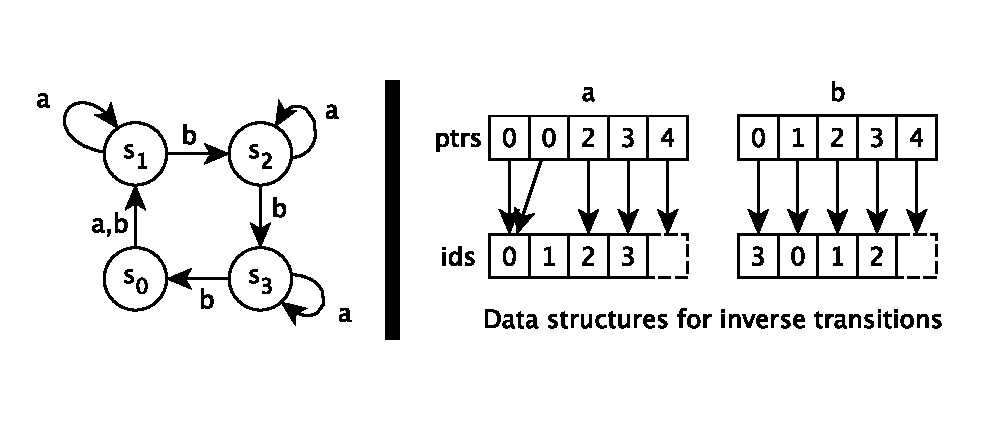
\includegraphics[width=0.9\textwidth]{figs/inverse.pdf}
	\caption{A synchronizing automaton ${\cal A}$~(left), and the data structures to store and process the transition function $\delta^{-1}$  in memory (right).
	For each state $s \in S$ and each input $x \in \Sigma$, {\tt ids}[{\tt ptrs}[$s$] $\cdots$ {\tt ptrs}[$s+1$] $ - 1$] store the ids for all states $s'$ such that $\delta(s',x) = s$.}
	\label{fig:inv}
\end{figure}

An element of the set $\Sigma^\star$ is called an {\em input sequence} (or simply {\em word}). $|w|$ denotes the length of $w$, and $\varepsilon$ expresses the empty word. The transition function $\delta$ can be extended to a set of states and to a word in the usual way. Assuming $\delta(s,\varepsilon)=s$, for a word $w \in \Sigma^\star$ and a letter $x \in \Sigma$, $\delta(s,xw) = \delta(\delta(s,x),w)$. Likewise, for a set of states $S' \subseteq S$, $\delta(S',w) = \{ \delta(s,w) | s \in S'\}$.

The inverse of the transition is also a well defined function; $\delta^{-1}(s,x)$ denotes the set of states with a transition to state $s$ with input $x$. Formally, $\delta^{-1}(s,x) = \{ s' \in S | \delta(s',x)= s\}$.  Figure~\ref{fig:inv}~(right) shows the data structure used to store the inverse transition function for the example automata.

Let ${\cal A}=(S, \Sigma, \delta)$, $C \subseteq S$ and $C^{\langle 2 \rangle} = \{ \{ s_i, s_j \}| s_i,s_j \in C \}$ be set of multisets  with cardinality two. For $\{ s_i, s_j \} \in C^{\langle 2 \rangle}$, if $s_i=s_j$ then it is called a \textit{singleton}, otherwise called a \textit{pair}. 

An automaton which is produced from the set of pairs; ${\cal A}^{\langle 2 \rangle}=(S^{\langle 2 \rangle},\Sigma,\delta^{\langle 2 \rangle})$ is called the \textit{pair automaton}. 
For a pair automaton, the set of inputs is the same and the transition function is $\delta^{\langle 2 \rangle}(\{ s_i,s_j \},x) = \{ \delta(s_i,x), \delta(s_j,x) \}$. 

\begin{figure}[ht]
	\centering
	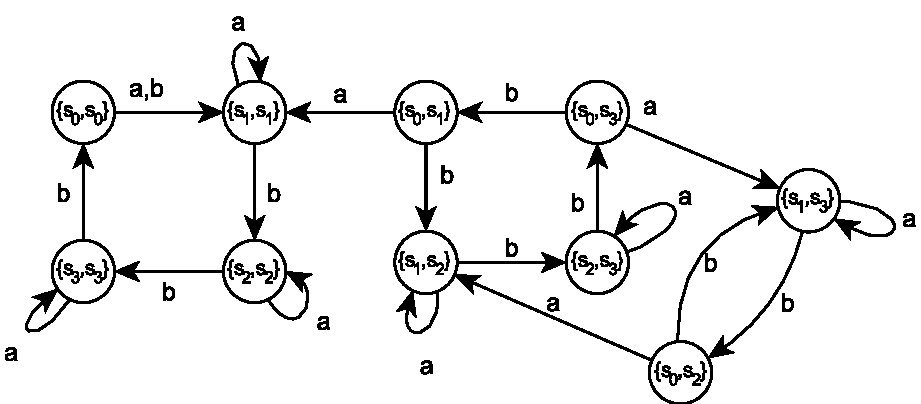
\includegraphics[width=\textwidth]{figs/pair.pdf}
	\caption{The pair automaton ${\cal A}^{\langle 2 \rangle}$ of the automaton in Figure \ref{fig:inv}.}
	\label{fig:pair}
\end{figure}

Let $C \subseteq S$ and $w \in \Sigma^*$, when cardinality of $\delta(C,w)$ is one then $w$ is a \textit{merging sequence} for $C$ and $C$ is called \textit{mergeable}. When $C=S$, $w$ is called a \textit{reset word} of automaton and the automaton is synchronizable. As shown by \cite{Eppstein90}, deciding if an automaton is synchronizing can be performed in time $O(pn^2)$ by checking if there exists a merging word for $\{ s_i, s_j \}$, for all  $\{ s_i, s_j \} \in S^{\langle 2 \rangle}$. 
Recently, Berlinkov \cite{Berlinkov2016} showed that there exist an algorithm that decides on synchronizability in linear expected time in $n$. 

\kkcomm{define Cerny automata here}

\clearpage
\section{Eppstein's \greedyAlgo\ Algorithm}
\label{sec:greedy}

The \greedyAlgo\ algorithm is one of the fastest algorithms among the reset word generation heuristics in the literature. The correctness of the algorithm is based on the following proposition.

\begin{proposition}
	\label{prop:synchronizable}
	An automaton ${\cal A}=(S,\Sigma,\delta)$ is synchronizing iff $\forall s_i,s_j \in S$, there exists a merging sequence for $\{ s_i, s_j \}$.
\end{proposition}

\noindent \greedyAlgo\  uses the shortest merging sequences of pairs to find a short reset word. Like most of the algorithms mentioned in Section \ref{sec:Intro}, \greedyAlgo\ has two  phases. In the first phase, it finds the shortest merging sequences for all pairs. If there is a pair which is not mergeable, due to Proposition~\ref{prop:synchronizable}, the automaton is not synchronizing. Otherwise, the algorithm continues with the second phase.

The merging sequences of pairs are stored in a function $\tau : S^{\langle 2 \rangle} \rightarrow \Sigma^\star$, which is called the \textit{pairwise merging function} (PMF) for ${\cal A}$. If $\{ s_i, s_j \}$ is mergeable, then $\tau(\{ s_i, s_j \})$ is the merging sequence, otherwise it is undefined. Note that PMF does not have to be unique, i.e., $\tau(\{ s_i, s_j \})$ may differ, however  $|\tau(\{ s_i, s_j \})|$ is unique and the shortest possible. To find all the shortest merging sequences, a breadth first search can be initiated over the pair automata. By using the inverse of transition function and starting from $\{ s_i, s_i \}$ singletons, all mergeable pairs and their shortest merging sequences can be found. Let $p=|\Sigma|$ and $n=|s|$; in worst case, the algorithm traverses all edges, i.e., $p$ letters of each $n(n-1)$ pairs and $n$ singletons should be checked. Therefore the complexity of the first phase is $O(pn^2)$. 

Algorithm \ref{algo:BFS} keeps the track of most recently computed mergeable pairs via a list, which is called \textit{frontier set} ($F$). The level of a frontier set refers the length of the corresponding merging sequences inside. Since $\tau(\{ s_i, s_i \})=\epsilon$, singletons are placed in the root level, level 0, of BFS. The \textit{rremaining set} ($R$) is the set of pairs whose merging sequences are not computed yet. At each iteration of Algorithm \ref{algo:BFS}, new frontier and remaining sets are computed for next level. 


\begin{algorithm}[ht]
	\caption{Computing a PMF $\tau : S^{\langle 2 \rangle} \rightarrow \Sigma^\star$}
	\label{algo:BFS}
	\SetKwInOut{Input}{input}\SetKwInOut{Output}{output}
	\Input{An automaton ${\cal A}=(S,\Sigma,\delta)$}
	\Output{A PMF $\tau : S^{\langle 2 \rangle} \rightarrow \Sigma^\star$}
	
	%compute the reverse automaton ${A}^{-1} = (S,\Sigma,\delta^{-1})$ of $A$\;
	\lForEach{singleton $\{ s,s \} \in S^{\langle 2 \rangle}$}{$\tau(\{ s,s \}) = \varepsilon$}
	\lForEach{pair $\{ s_i,s_j \} \in S^{\langle 2 \rangle}$}{$\tau(\{ s_i,s_j \}) =$ {\em undefined}}
	
	$F \longleftarrow \{ \{ s,s \} | s \in S \}$; \tcp{all singletons of $S^{\langle 2 \rangle}$}
    $R \longleftarrow \{ \{ s_i, s_j \} | s_i,s_j \in S \wedge s_i \neq s_j \}$; \tcp{all pairs of $S^{\langle 2 \rangle}$}
	\While{$R$ is not empty and $F$ is not empty}
	{
		$F,R,\tau \longleftarrow \mbox{BFS\_step}(A,F,R,\tau)$\;
	}
\end{algorithm}

\begin{proposition}
	\label{prop:merging}
	Let $\{ s_i,s_j \}$ be a pair in $S^{\langle 2 \rangle}$. If $w \in \Sigma^*$ is a merging sequence for $\delta(\{ s_i,s_j \}, x)$ then $xw$ is a merging sequence for $\{s_i,s_j \}$.
\end{proposition}

Thanks to the inverse of transition function and Proposition \ref{prop:merging}, Algorithm \ref{algo:BFS-step-F2R} constructs PMF from the most recent frontier set. At lines 3-4, the algorithm searches the pairs which can reach the frontier set pairs by applying a single letter. When the algorithm finds such a pair whose merging sequence has not been defined yet, it marks the pair as the next frontier set's pair for the next iteration and sets its merging sequence. Since the algorithm computes the PMF of the remaining set by using the frontier set, it is called \textit{frontier to remaining} (F2R). 

\begin{algorithm}[ht]
	\caption{{BFS\_step (F2R)}}
	\label{algo:BFS-step-F2R}
	
	\SetKwInOut{Input}{input}\SetKwInOut{Output}{output}
	\Input{An automaton ${\cal A}=(S,\Sigma,\delta)$, the frontier $F$, the remaining set $R$, $\tau$}
	\Output{The new frontier $F'$, the new remaining set $R'$, and updated function $\tau$}
	
	$F' \longleftarrow \emptyset$\;
	\ForEach{$ \{ s_i,s_j \} \in F$}
	{
		\ForEach{$x \in \Sigma$}
		{
			\ForEach{$\{ s'_i,s'_j\}$ such that $s'_i \in \delta^{-1}(s_i,x)$ and $s'_j \in \delta^{-1}(s_j,x)$}
			{
				\If(\tcp*[h]{$\{ s'_i,s'_j\} \in R$}){$\tau(\{ s'_i,s'_j\})$ is undefined}
				{
					$\tau(\{ s'_i,s'_j \}) \longleftarrow x \tau(\{ s_i,s_j \})$\;
					$F' = F' \cup \{ \{ s'_i,s'_j \}  \} $\;
				}
			}
		}
	}
	let $R'$ be $R \setminus F'$;
\end{algorithm}

When the first phase is completed, Algorithm \ref{algo:greedy} first checks if the automaton is synchronizing or not in $O(n^2)$ (lines 2-3). It then initializes the \textit{set of active states} ($C$) as the set of all states and the initial reset word as empty. After that, iteratively, it selects the shortest merging sequence of all active pairs, appends it to reset word, and finally updates the set of active states by applying the selected merging sequence. This operation is repeated until only a single active state is left. 

At each iteration, the merging sequence is applied, so the cardinality of $C$ decreases. Therefore at most $n-1$ iterations are performed. At line 7, the algorithm finds the active pair with the shortest merging sequence which takes $O(n^2)$ per iteration. Line 8 takes constant time. The length of each merging sequence can be at most $n^2$. Therefore the time complexity of line 9 is $O(n^3)$ for a single iteration. Overall, the second phase takes $O(n^4)$ and Algorithm \ref{algo:greedy} requires $O(pn^2 + n^4)$ time. 

The upper bounds of the phases can be computed in a slightly different way. For a synchronizing automaton, the first phase is $\Omega(n^2)$ since it finds a merging sequence for all pairs. At best, phase two takes a merging sequence with length of one, which is also a reset word. Then the algorithm applies the merging sequence to all states. Therefore, the lower bound of the second phase is $\Omega(n)$. Thus Algorithm \ref{algo:greedy} has $O(pn^2 + n^4)$ and $\Omega(n^2)$ time complexity. Since there is a huge gap between the best  and the worst case complexities, we extended our observations with the empirical results. In the next subsection, the bottleneck of the algorithm is introduced with a thorough experimental analysis.

\begin{algorithm}[ht]
	\caption{Eppstein's \greedyAlgo\ algorithm}
	\label{algo:greedy}
	
	\SetKwInOut{Input}{input}\SetKwInOut{Output}{output}
	\Input{An automaton ${\cal A}=(S,\Sigma,\delta)$}
	\Output{A reset word $\Gamma$ for ${\cal A}$ (or fail if ${\cal A}$ is not synchronizable)}
	
	%{--- Phase 1 ---}
	compute a PMF $\tau$ using Algorithm~\ref{algo:BFS}\;
	\If{there exists a pair $\{ s_i,s_j \}$ such that  $\tau(\{ s_i,s_j \})$ is undefined}
	{
		report that ${\cal A}$ is not synchronizable and exit;	
	}

	
	%{--- Phase 2 ---}
	$C = S$; \tcp{$C$ will keep track of the current set of states}
	$\Gamma = \varepsilon$; \tcp{$\Gamma$ is the synchronizing sequence to be constructed}
	
	\While(\tcp*[h]{we have two or more states yet to be merged}){$|C| > 1$}
	{
		$\{ s_i,s_j \} = Find\_Min(C, \tau)$\;
		
		
		$\Gamma = \Gamma \; \tau(\{ s_i,s_j \})$\;
		$C = \delta(C,\tau(\{ s_i,s_j \}))$;
	}
\end{algorithm}


\begin{algorithm}[ht]
	\caption{Find\_Min}
	\label{algo:find-min}
	
	\SetKwInOut{Input}{input}\SetKwInOut{Output}{output}
	\Input{Current set of state $C$ and the PMF function $\tau$}
	\Output{A pair of state $\{ s_i,s_j \}$ with minimum $|\tau(\{ s_i,s_j \})|$ among all pairs in $C^{\langle 2 \rangle}$}
	
	$\{ s_i,s_j \} =$ undefined\;
	\ForEach{$ \{ s_k,s_\ell \} \in C^{\langle 2 \rangle}$}
	{
		\If{$\{ s_i,s_j \}$ is undefined or $|\tau(\{ s_k,s_\ell \})| < |\tau(\{ s_i,s_j \})|$}
		{
			$\{ s_i,s_j \} = \{ s_k, s_\ell \}$
		}
	}
\end{algorithm}



\subsection{Analysis on \greedyAlgo}
\label{sec:greedy-analysis}

As discussed in Section \ref{sec:greedy}, the time complexity of \greedyAlgo\ is $O(pn^2 + n^4)$. For most of the cases, $p$ is too small when compared to $n$. Hence, the complexity of the second phase, $O(n^4)$, dominates the first phase in theory. To analyze the algorithm, we performed experiments on 100 randomly generated automata for each  $p \in \{2, 8, 32, 128\}$ letters and  $n \in \{2000, 4000, 8000\}$ states. In addition, we used \v{C}ern\'y automata \kkcomm{we need the definition in the previous section} \cite{cerny} for $n \in \{2000, 4000, 8000\}$ states. In Table \ref{table:phase-comparison}, experiments from 1200 randomly generated automata show that the execution time of the second phase does not dominate the overall time of the algorithm for random automata.

\begin{table}[ht]
	\center
	\scalebox{0.89}{
		\begin{tabular}{r|rrr|rrr|rrr}
		&\multicolumn{3}{|c}{$n = 2000$}&\multicolumn{3}{|c}{$n = 4000$}&\multicolumn{3}{|c}{$n = 8000$}\\
		$p$ & $t_{PMF}$ & $t_{ALL}$ & $\frac{t_{PMF}}{t_{ALL}}$ & $t_{PMF}$ & $t_{ALL}$ & $\frac{t_{PMF}}{t_{ALL}}$ & $t_{PMF}$ & $t_{ALL}$ & $\frac{t_{PMF}}{t_{ALL}}$\\\hline
			2		& 0.172	& 0.185	& 0.929	& 1.184		& 1.240		& 0.954	& 5.899		& 6.325		& 0.933 \\
			8		& 0.504	& 0.517	& 0.975	& 2.709		& 2.768		& 0.978	& 14.289	& 14.721	& 0.971 \\
			32		& 2.113	& 2.126	& 0.994	& 9.925		& 9.986		& 0.994	& 51.783	& 52.233	& 0.991 \\
			128		& 9.126	& 9.140	& 0.999	& 40.356	& 40.418	& 0.998	& 193.548	& 193.982	& 0.998 \\
			\v{C}ern\'y	& 0.096	& 4.836	& 0.020	& 1.026		& 42.771	& 0.024	& 5.584		& 797.692	& 0.007
		\end{tabular}
	}
	\caption{Sequential PMF construction time ($t_{PMF}$), and overall time ($t_{ALL}$) in seconds}
	\label{table:phase-comparison}
\end{table}

To understand the behavior of the algorithm, we extended our experiments by analyzing the structure of PMF. While computing time complexity of the algorithm, the length of the merging sequence is at most $n^2$. However, Table \ref{table:levels} shows that $n^2$ is loose bound for the length of merging sequence. For instance, when automata with 8000 states and 128 letters are considered, the lengths of merging sequences in PMF are at most 3, not 64000000. Another observation is that the second phase tends to pick shorter length of merging sequences. For example, when we take an automaton with 8000 states and 2 letters, the longest merging sequence in PMF has the length 16.9. The second phase uses only merging sequences with length 12.1 and less. Thus, the merging sequences of almost 30\% of the nodes are not necessarily computed (see Figure \ref{fig:nodes-at-levels}).

\begin{table}[ht]
	\center
	\begin{tabular}{r|rrr|rrr|rrr}
 		& \multicolumn{3}{c|}{n=2000} & \multicolumn{3}{c|}{n=4000} & \multicolumn{3}{c}{n=8000} \\
		p &  $h_{PMF}$ &  $h_{max}$ &  $h_{mean}$ &  $h_{PMF}$ &  $h_{max}$ &  $h_{mean}$ &  $h_{PMF}$ &  $h_{max}$ &  $h_{mean}$ \\ \hline
 		2 &  14.2 &  10.0 &  1.9 &  15.5 &  11.2 &  1.9 &  16.9 &  12.1 &  1.9 \\
 		8 &  5.0 &  4.0 &  1.3 &  6.0 &  4.2 &  1.3 &  6.0 &  4.6 &  1.3 \\
		32 &  3.1 &  2.7 &  1.1 &  4.0 &  2.9 &  1.1 &  4.0 &  3.0 &  1.1 \\
		128 &  3.0 &  2.0 &  1.0 &  3.0 &  2.0 &  1.0 &  3.0 &  2.1 &  1.0 \\
%		\v{C}ern\'y & 1999000.0 & 1952000.0 & 8884.8 & 7998000.0 & 7808000.0 & 19750.8 & 31996000.0 & 31232000.0 & 43480.8
		\v{C}ern\'y & $2.0\times10^6$ & $2.0\times10^6$ & $8.8\times10^3$ & $8.0\times10^6$ & $7.8\times10^6$ & $2.0\times10^4$ & $3.2\times10^7$ & $3.1\times10^7$ & $4.3\times10^4$
	\end{tabular}
	\caption{The length of longest merging sequence in PMF($h_{PMF}$) constructed in Phase 1; maximum ($h_{max}$), and average ($h_{mean}$) lengths for merging sequences, used in the second phase of \greedyAlgo. \comment{sertac}{cerny deney sonuclari cok uzun oldu. yeni tabloya mi koysam? yoksa kuculteyim mi?}}
	\label{table:levels}
\end{table}

\begin{figure}[ht]
	\centering
	\subfigure[$p = 2$]{
		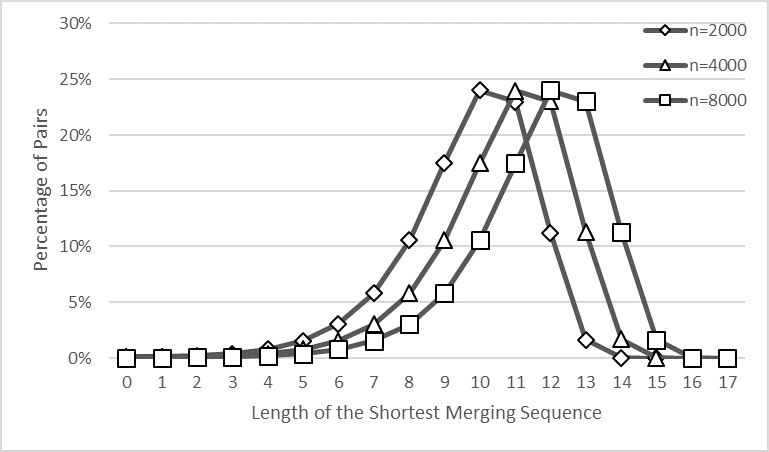
\includegraphics[width=0.47\textwidth]{figs/node_2.png}
	}
	\subfigure[$p = 8$]{
		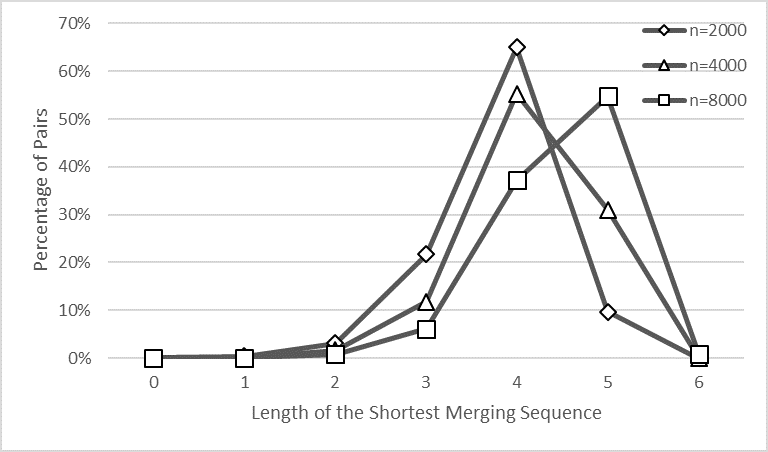
\includegraphics[width=0.47\textwidth]{figs/node_8.png}
	}
	\subfigure[$p = 32$]{
		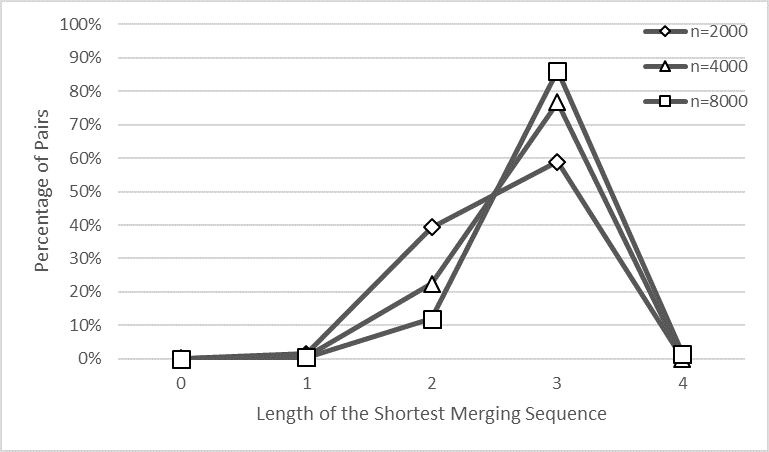
\includegraphics[width=0.47\textwidth]{figs/node_32.png}
	}
	\subfigure[$p = 128$]{
		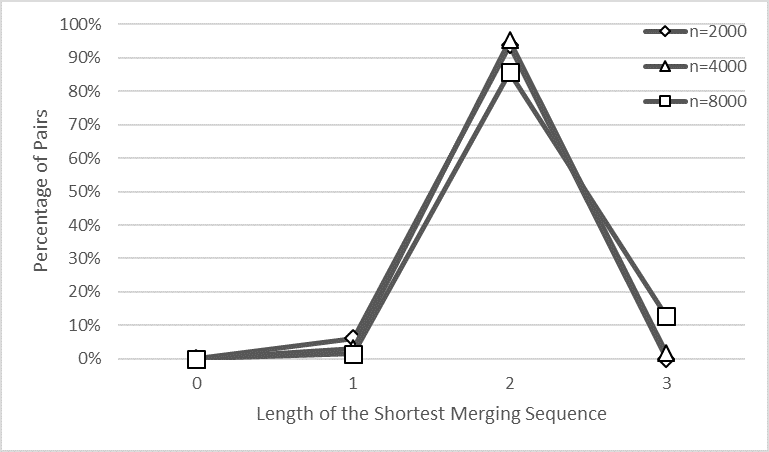
\includegraphics[width=0.47\textwidth]{figs/node_128.png}
	}
	\caption{The percentage of nodes at each level in PMF}
	\label{fig:nodes-at-levels}
\end{figure}


With these experiments, we observed that the execution time of PMF construction phase in general dominates the \greedyAlgo\ algorithm except some special automata classes such as \v{C}ern\'y. Therefore, we focused on parallelization of PMF construction, which is explained in Section \ref{sec:parallel}. We also noticed that not all information from the first phase is used in the second phase. Based on these observations, various algorithmic improvements that make \greedyAlgo\  much faster are presented in Section \ref{sec:speedup}. But first, we will focus on its parallelization in the next section.


%%%%%%%%%%%%% PARALLEL %%%%%%%%%%%%%%  
\clearpage
\section{Parallelization on \greedyAlgo}
\label{sec:parallel}

Our preliminary experiment results show that in general, the PMF construction phase is the bottleneck of \greedyAlgo. The first approach we took to reduce its cost is using parallel algorithms. 

Algorithm \ref{algo:BFS} is a BFS-like algorithm which starts from singletons and searches the shortest merging sequences of all pairs. The length of the merging sequence for a pair represents the level of the pair in BFS tree. Since the merging sequence of each singleton is $\epsilon$, the algorithm initially sets singletons as level 0 nodes. To find the $k^{th}$ level nodes, Algorithm \ref{algo:BFS-step-F2R} uses the $k-1^{st}$ level as the frontier set. The cost of processing each pair in the frontier set depends on the cost of inverse transition function $\delta^{-1}$. Likewise, the cost of each iteration depends on the number of pairs in frontier set. Therefore, the cost in each iteration vary.

\subsection{Frontier to Remaining in Parallel}
\label{sec:BFS-F2R-parallel}

While finding the $k^{th}$ level pairs (in the next frontier set $F'$), the algorithm has to ensure that all pairs from the $(k-1)^{st}$ level are found. Likewise, for correctness, it needs to process all $k^{th}$ level pairs before processing a pair from the $(k+1)^{st}$ level. Hence, a FIFO-based data structure satisfies these requirements. Since the sequential implementation picks a single pair at a time, a simple queue is more than enough to schedule processing of pairs. 

Indeed, using a queue is a flawless method to maintain the dependency between the pairs. However, implementing a parallel version of the algorithm is not that straightforward. Each thread needs to processes the pairs from the same level; otherwise, a pair from the next frontier can be processed before another pair in the current frontier and an incorrect PMF can be computed. The problem can be solved if the queue is implemented in a thread-safe manner; that is concurrent insertions and deletions cannot disrupt the integrated FIFO strategy. However, such an implementation requires expensive synchronization mechanisms such as atomic operations and locks. Since there can be millions of enqueue and dequeue operations to be performed, the queue itself will be the bottleneck. Fortunately, we do not have any restriction on the processing order of the pairs in the same level and a cheaper parallelization approach exists.  

\begin{algorithm}[ht]
	\caption{BFS\_step\_F2R (in parallel)}
	\label{algo:BFS-step-F2R-Parallel}
	
	\SetKwInOut{Input}{input}\SetKwInOut{Output}{output}
	\Input{An automaton ${\cal A}=(S,\Sigma,\delta)$, the frontier $F$, the remaining set $R$, $\tau$}
	\Output{The new frontier $F'$ and updated function $\tau$}
	
	\lForEach{thread $t$}{
		$F'_t \longleftarrow \emptyset$
	}
	\ForEachP{$\{ s_i,s_j\} \in F$}
	{
		\ForEach{$x \in \Sigma$}
		{
			\ForEach{$\{ s'_i,s'_j\}$ where $s'_i \in \delta^{-1}(s_i,x)$ and $s'_j \in \delta^{-1}(s_j,x)$}
			{
				\If(\tcp*[h]{$\{ s'_i,s'_j\} \in R$}){$\tau({\{ s'_i,s'_j \}})$ is undefined}
				{
					$\tau(\{ s'_i,s'_j\}) \longleftarrow x \tau(\{ s_i,s_j \})$\;
					$F'_t = F'_t \cup \{ \{ s'_i,s'_j \}  \} $\;
				}
			}
		}
	}
	$F' \longleftarrow \emptyset$\;
	\lForEach{thread t}{
		$F' = F' \cup F'_t$
	}
	let $R'$ be $R \setminus F'$;
\end{algorithm}

The parallel implementation is presented in Algorithm \ref{algo:BFS-step-F2R-Parallel}. In this algorithm, each pair in $F$ is assigned to a single thread. When a thread finds a new pair whose merging sequence is not decided yet, it pushes it to the new frontier set. Since pushing an item to a set is not an atomic operation, we need to change the process of insertions to the next frontier set. The easiest way is considering the process as a critical region~(which can be executed only a single thread at a time). However, as mentioned before, this is not time efficient. Here we implemented a lock-free mechanism. Instead of global $F'$, each thread stores a local $F'$. When all pairs from $F$ are processed, a thread merges local sets $F'$ in a sequential manner. Yet, this lock-free mechanism comes with a drawback. If two threads find the same pair at the same time, which is possible due to concurrency, both threads push it to $F'$ (lines 5-6 of Algorithm \ref{algo:BFS-step-F2R-Parallel}). Hence, the same pair can exist multiple times in the combined frontier. One can solve this problem with a separate duplicate pair removal process which can be a burden on the performance. For CPU parallelization, our preliminary experiments revealed that at most one in a thousand extra pairs are inserted to $|F'|$. Since duplicate pairs do not effect the correctness of the algorithm, we decided not to perform a costly duplicate pair elimination. Instead, the algorithm processes them more than once whose time cost is negligible. 

Due to duplicate pairs, updating the remaining pair set $R$ becomes a costly operation. In the sequential implementation of Algorithm \ref{algo:BFS}, we were just counting the number of remaining pairs, i.e., $|R|$. However, in the parallel version, correctly counting the number of remaining pairs while allowing duplicate pairs is not possible. A careless implementation can think that all the pairs are processed even if some are still existing. Therefore, in parallelization of Algorithm \ref{algo:BFS}, we do not maintain $R$. Instead, we allow the implementation perform one more iteration in which no updates are detected. Although this approach requires an extra iteration, its cost is also negligible compared to the cost of maintaining $R$.

\subsection{Remaining to Frontier}
\label{sec:BFS-R2F-parallel}

Using the frontier set $F$ to construct PMF, like in Algorithm \ref{algo:BFS-step-F2R} and \ref{algo:BFS-step-F2R-Parallel}, is the most natural and common way for a BFS algorithm. Another approach is using the remaining set $R$ to construct PMF which we called as \textit{remaining to frontier} (R2F). The main difference is that R2F uses transition function $\delta$ as edges, compared to F2R uses $\delta^{-1}$. Thanks to Proposition \ref{prop:merging}, Algorithm \ref{algo:BFS-step-R2F-Parallel} searches all pairs $\{ s_i,s_j \}\in R$ and applies all possible letters $x \in \Sigma$. If the algorithm finds a merging sequence $\delta(\{ s_i,s_j \}, x) = w$ (lines 4-6), then it sets $\tau(\{ s_i,s_j \}) = xw$ (lines 7-9). Otherwise, the pair is pushed to $R'$ (lines 10, 11). Similar to Algorithm \ref{algo:BFS-step-F2R-Parallel}, Algorithm \ref{algo:BFS-step-R2F-Parallel} also uses local sets. Each thread $t$ uses its local next remaining set $R'_t$ for lock-free parallelization. Note that, each thread processes different pairs $\{ s_i,s_j \}$. Hence, there is no duplicate pairs in $R'$. Algorithm \ref{algo:BFS} can use $R$ and iterates one less compared to parallel version of F2R.

\begin{algorithm}[ht]
	\caption{BFS\_step\_R2F (in parallel)}
	\label{algo:BFS-step-R2F-Parallel}
	
	\SetKwInOut{Input}{input}\SetKwInOut{Output}{output}
	\Input{An automaton ${\cal A}=(S,\Sigma,\delta)$, the frontier $F$, the remaining set $R$, $\tau$}
	\Output{The new frontier $F'$, the new remaining set $R'$, and updated function $\tau$}
	
		\lForEach{thread t}{$R'_t \longleftarrow \emptyset$}
		\ForEachP{$\{ s_i,s_j \} \in R$}
		{
			$connected  \longleftarrow $ {\bf false}\;
			\ForEach{$x \in \Sigma$}
			{
				$\{ s'_i, s'_j \}\longleftarrow \{ \delta(s_i,x),\delta(s_j,x) \}$; \\ 

				\If(\tcp*[h]{$\{ s'_i,s'_j\} \in F$}){$\tau(\{ s'_i, s'_j \})$ is defined}
				{
					$\tau( \{ s_i, s_j\}) \longleftarrow x \tau(\{ s'_i, s'_j \})$\;
					$connected  \longleftarrow $ {\bf true}\;
					{\bf break}\;
				}
			}
			\If{not $connected$}
			{
					$R'_t = R'_t \cup \{ \{ s_i, s_j \} \} $\;
			}
		}
		$R' \longleftarrow \emptyset$\;
		\lForEach{thread t}{
			$R' = R' \cup R'_t$
		}
	let $F'$ be $R \setminus R'$;
\end{algorithm}


\subsection{Hybrid Approach}
\label{sec:BFS-Hybrid-parallel}
The costs of Algorithm \ref{algo:BFS-step-F2R-Parallel} and \ref{algo:BFS-step-R2F-Parallel} are closely related to the size of frontier set $F$ and remaining set $R$ respectively. Initially $R$ is set of all pairs and $F$ is set of all singletons. The size of $R$ decreases by the size of $F$ at each iteration. Our preliminary observations, like in Figure \ref{fig:BFS-vtcomparison}, also indicates that the size of $R$ is bigger than the size of $F$ in early stages, but at later iterations the situation becomes contrary. At each iteration of PMF construction, it is possible to predict the cost of F2R and R2F algorithms which allows us to choose the algorithm with less cost in a hybrid manner at each iteration. 


\begin{figure}[ht]
	\centering
	\subfigure[$p = 8$, \# of vertices]{
		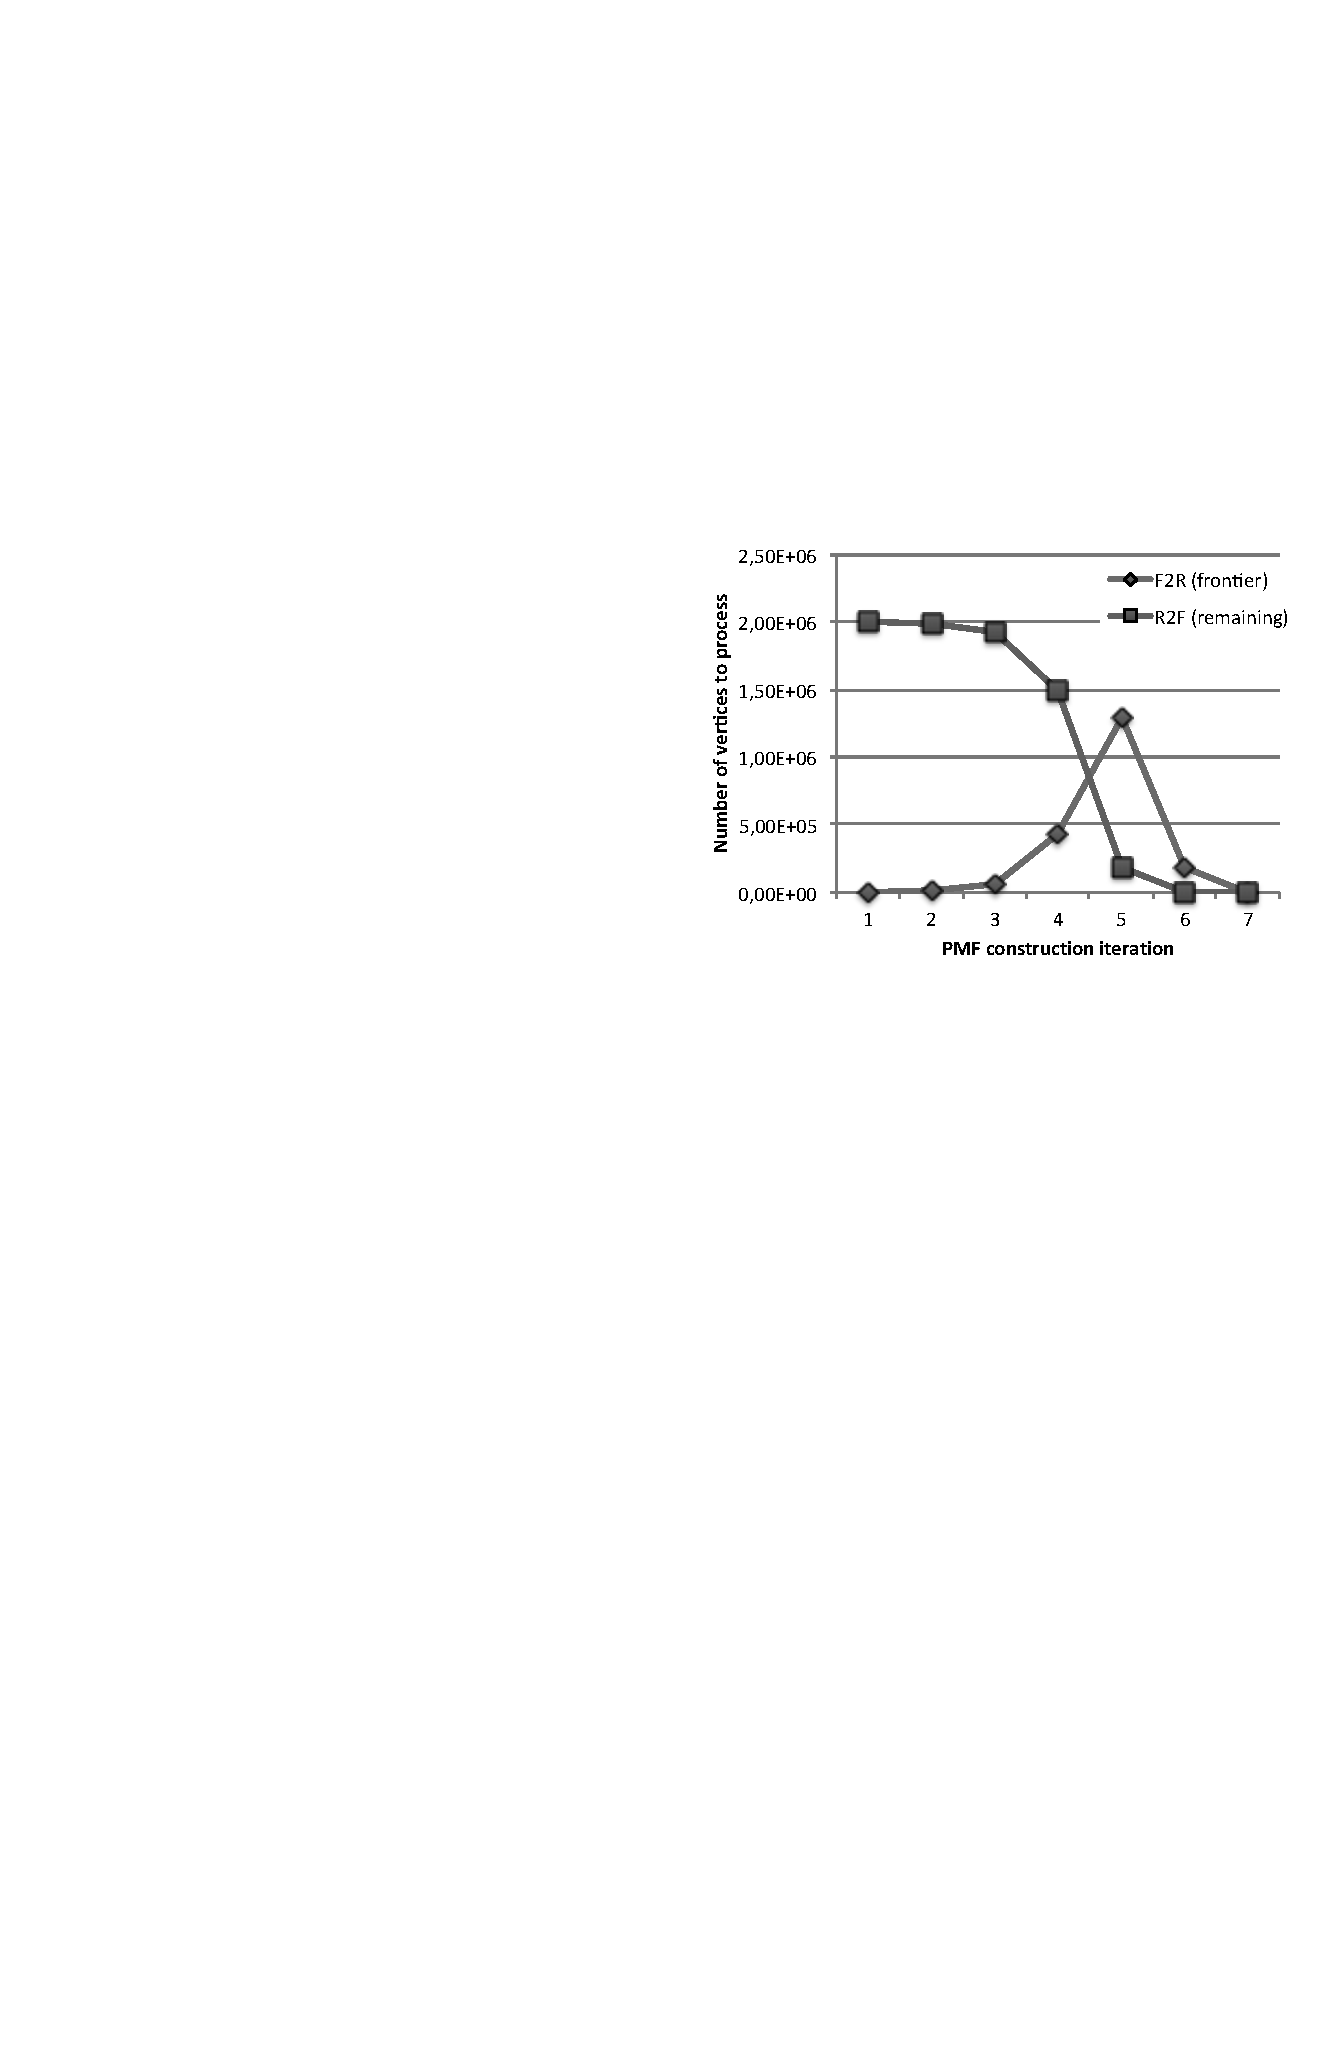
\includegraphics[width=0.44\textwidth]{figs/8v_gray.pdf}
	}
	\subfigure[$p = 8$, execution time]{
		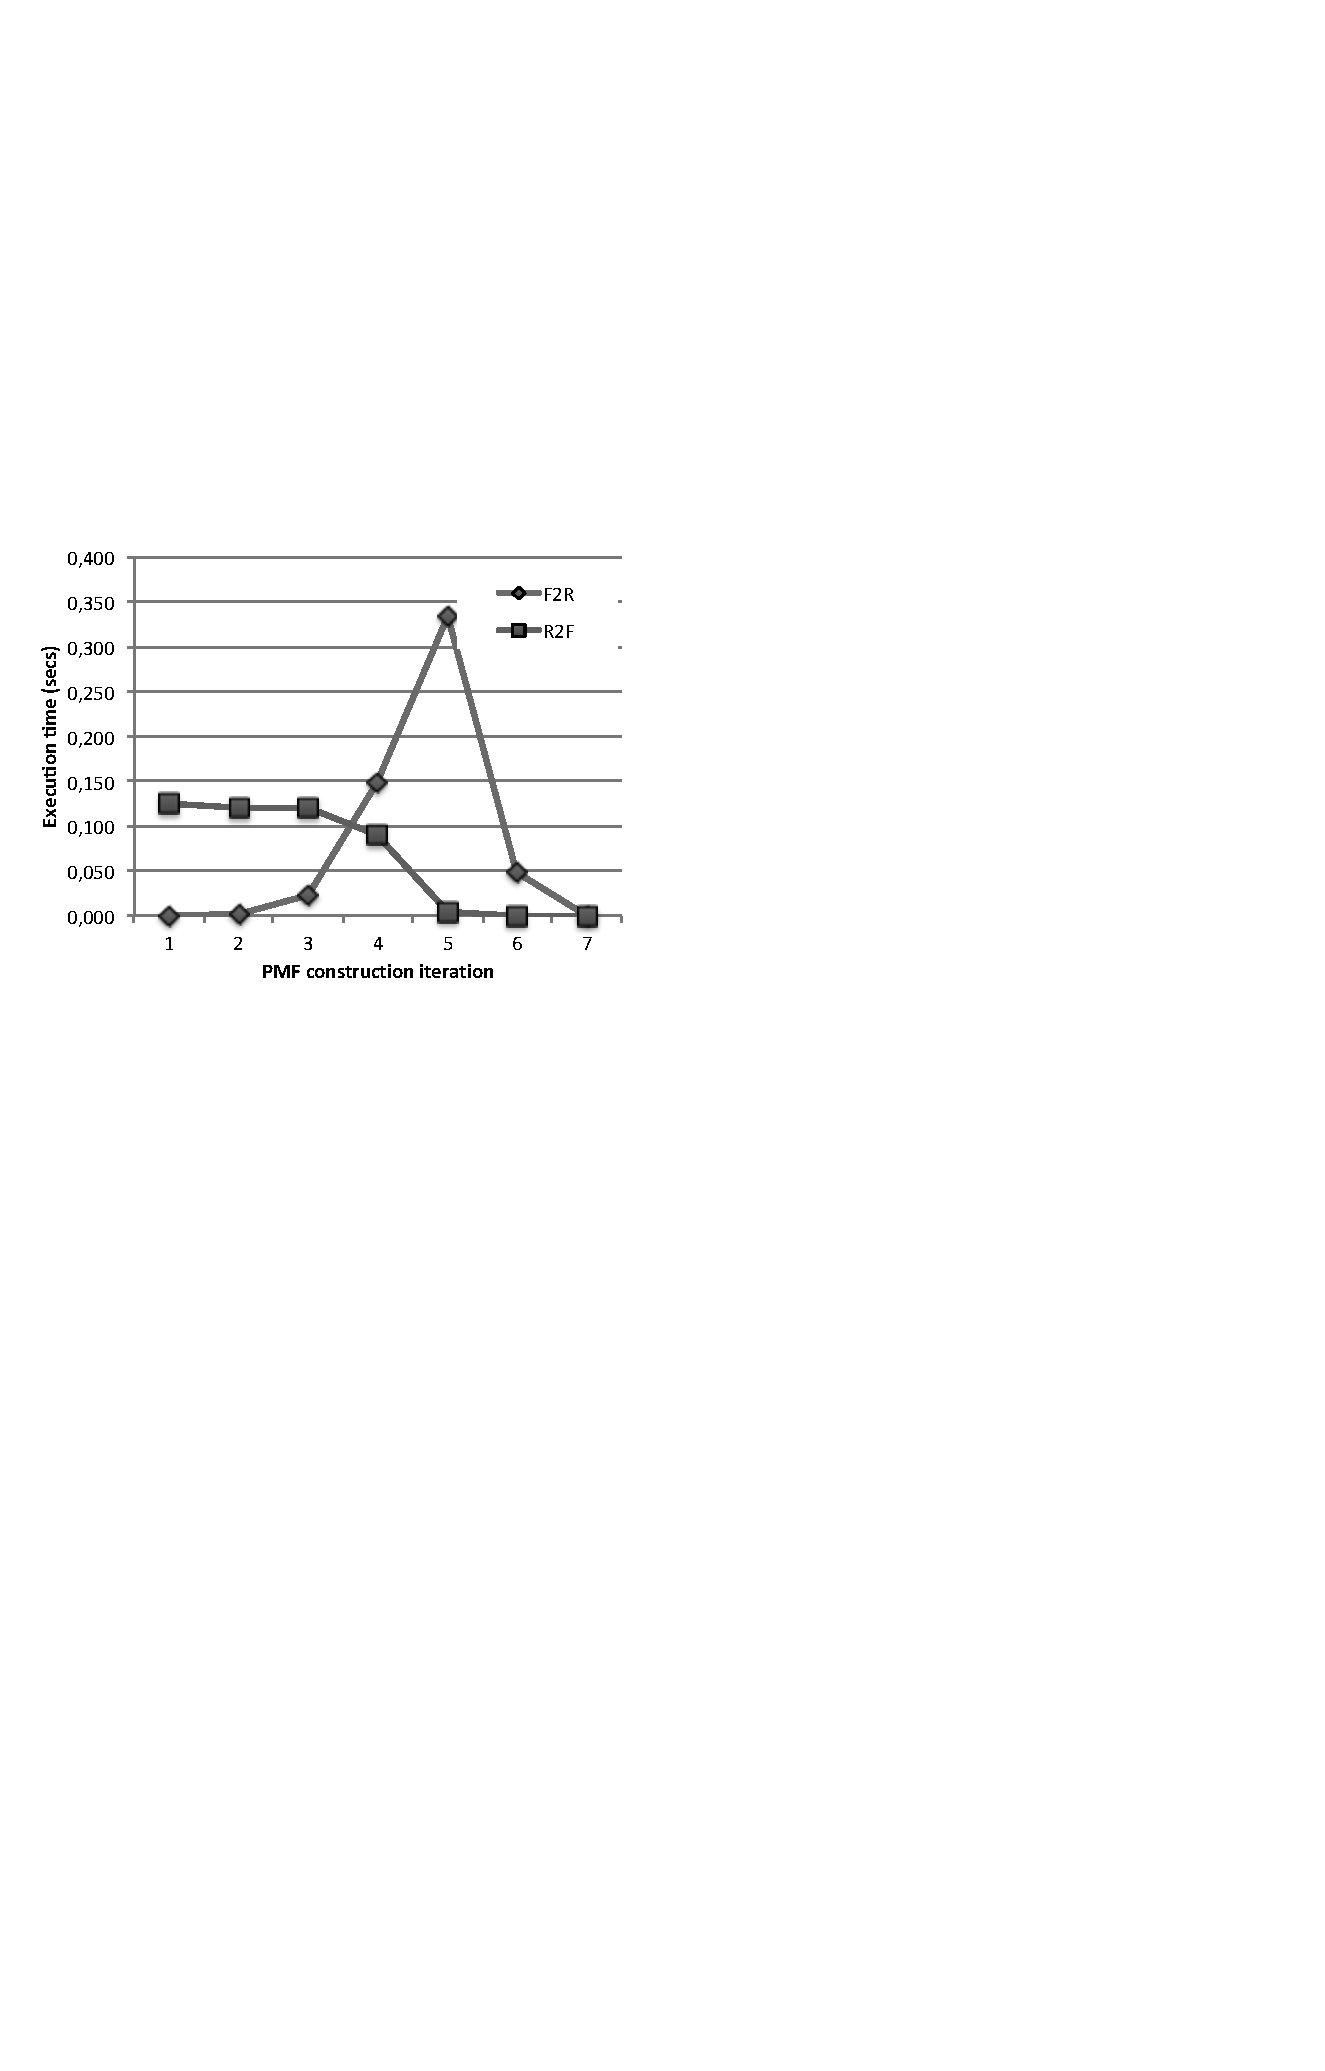
\includegraphics[width=0.44\textwidth]{figs/8t_gray.pdf}
	}
	\quad
	\subfigure[$p = 128$, \# of vertices]{
		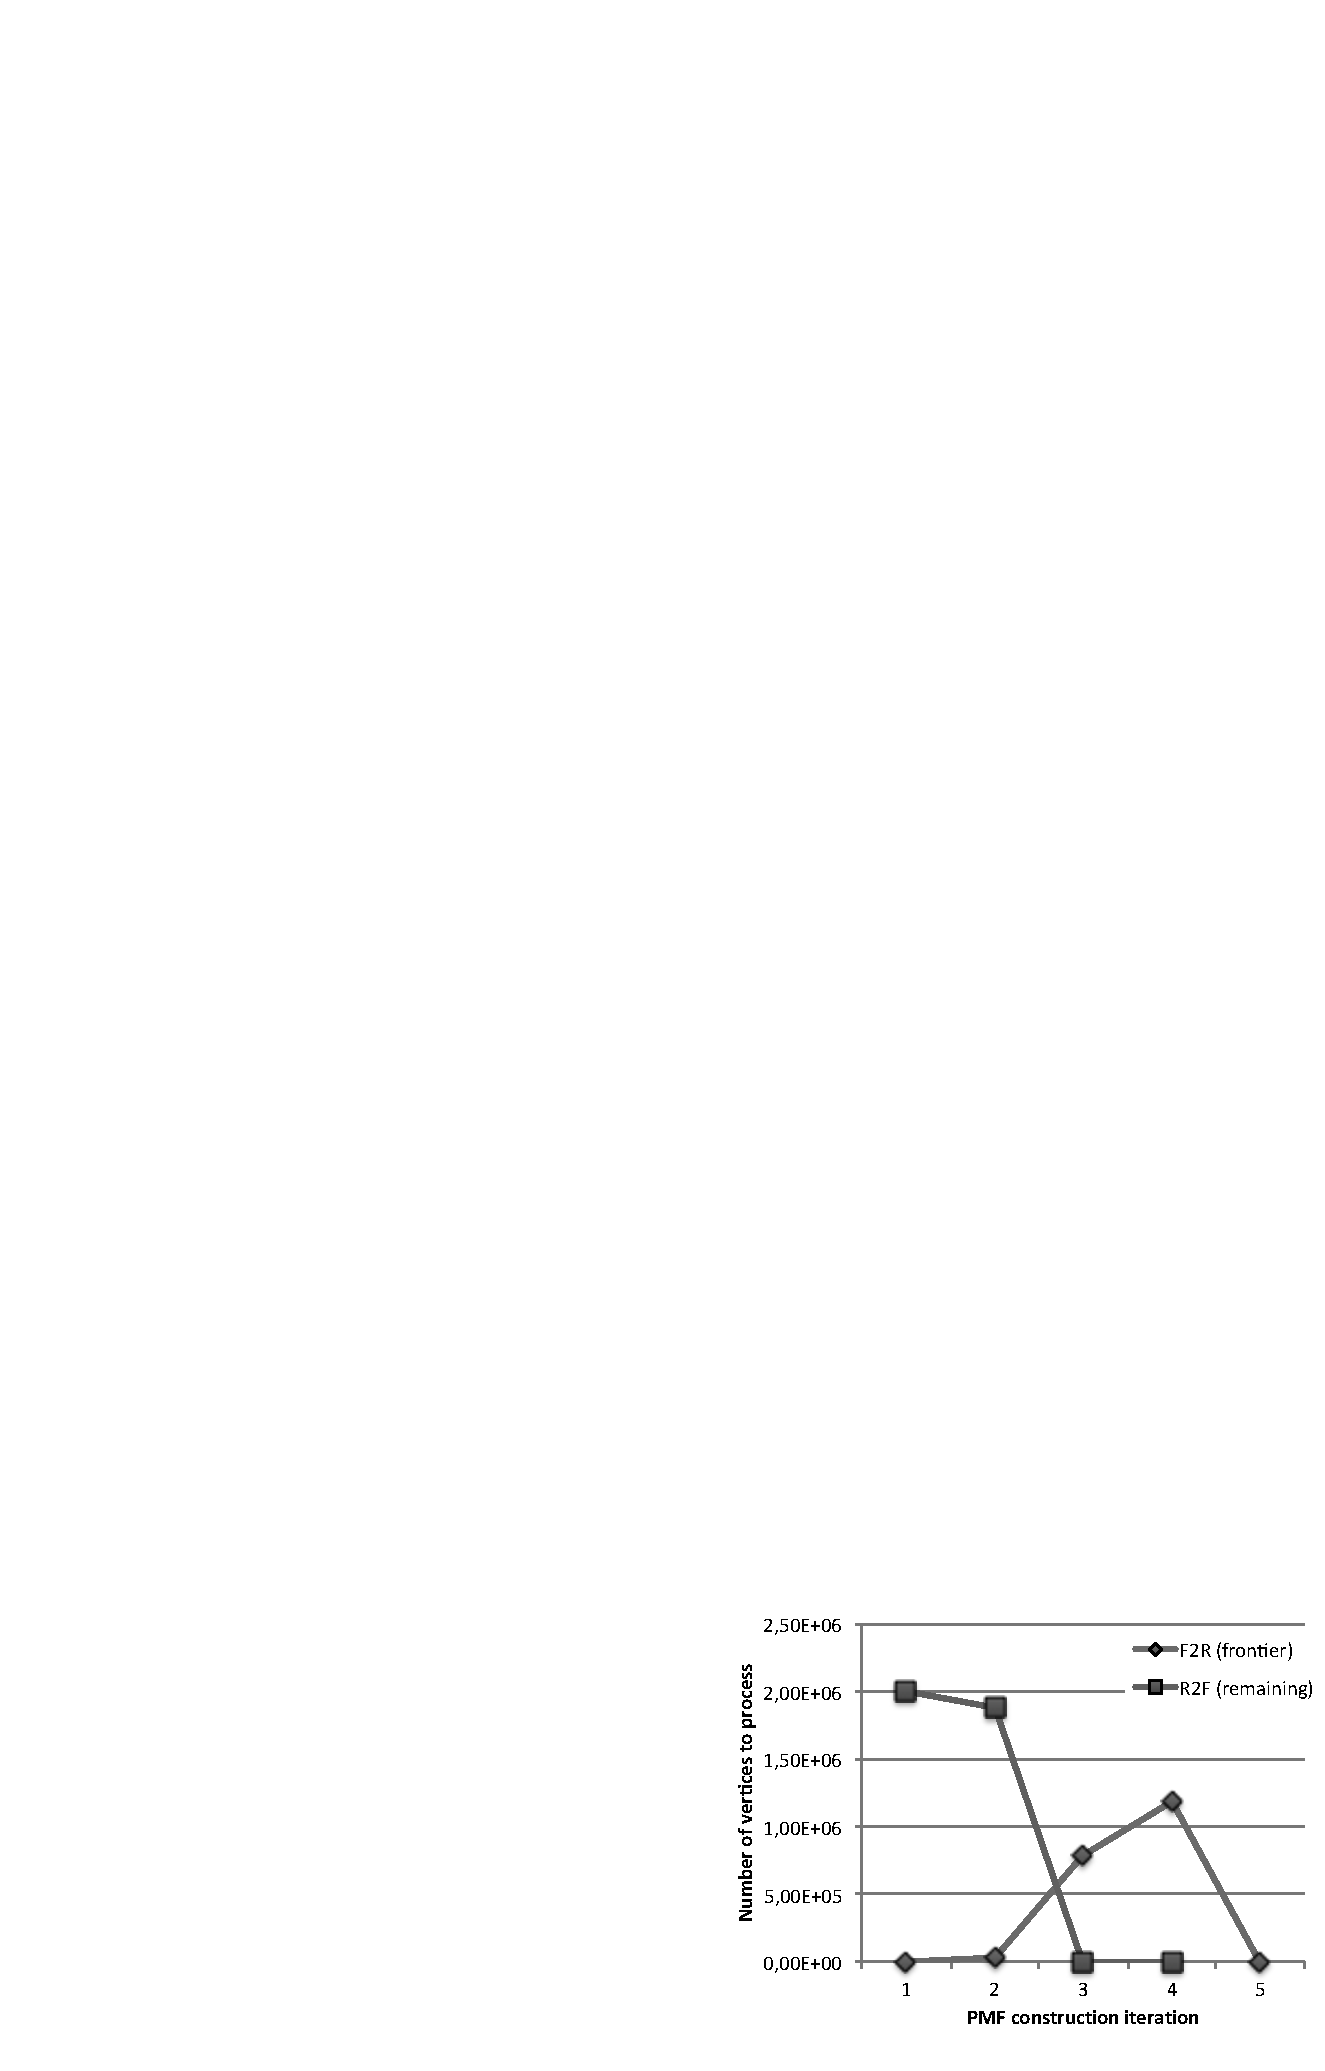
\includegraphics[width=0.44\textwidth]{figs/128v_gray.pdf}
	}
	\subfigure[$p = 128$, execution time]{
		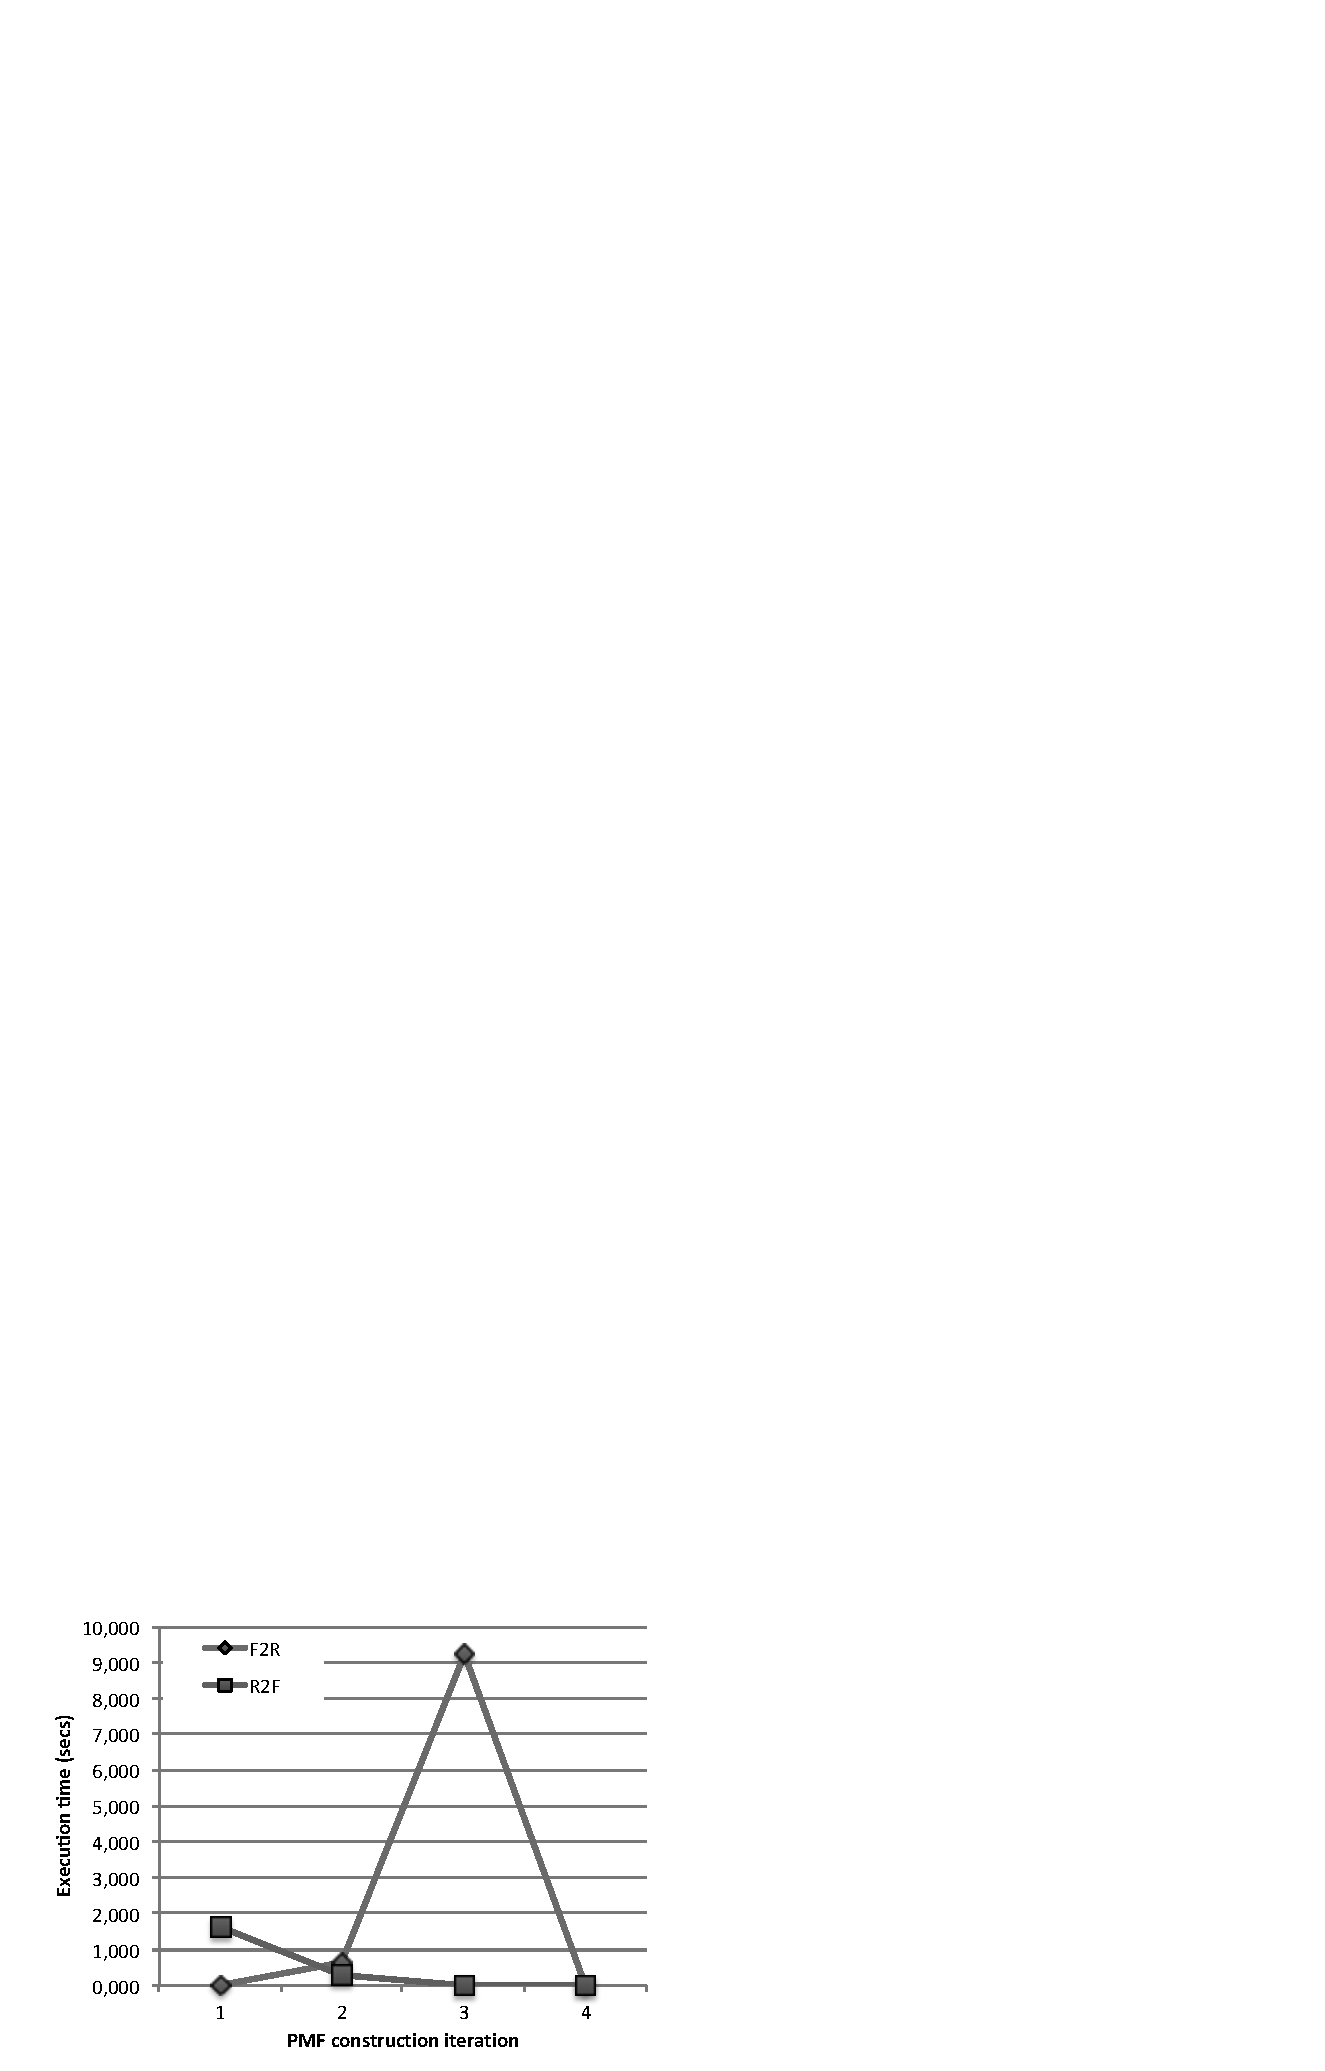
\includegraphics[width=0.44\textwidth]{figs/128t_gray.pdf}
	}
	\caption{The number of frontier and remaining vertices at each BFS level and the corresponding execution times of F2R and R2F while constructing the PMF $\tau$ for $n = 2000$ and $p = 8$~(top) and $p=128$~(bottom). 
\comment{sertac}{sayilardaki virguller nokta olmali.}}%As described above, F2R processes the edges of the frontier vertices at each level, whereas R2F processes those of the remaining vertices.
	
	\label{fig:BFS-vtcomparison}
\end{figure}

The idea of hybrid approach in BFS algorithm is introduced by Beamer et al. \cite{Beamer}. The algorithm checks all edges, so determining the cost of each iteration by the number of edge is the most precise technique as in \cite{Beamer}. On a simple graph, counting the edges is an effortless operation. However in our work, the BFS algorithm is applied to a pair automaton ${\cal A}^{\langle 2 \rangle}$ which is not actually created. For each pair it requires $O(p)$ time to count number of edges for F2R. Accordingly, estimating the cost of F2R and R2F from edges takes $O(pn^2)$ which is the same time complexity of the BFS algorithm itself. For R2F, the number of edge per vertex is fixed to alphabet size. For F2R, the number of edge per vertex varies. However the average value is equal to alphabet size, like in R2F. Therefore assuming the number of edge per vertex approximately equals to the alphabet size is a fine acceptance. Thus one can use the number of vertices to predict the cost of the algorithms.



\begin{algorithm}[ht]
	\label{algo:BFS-Hybrid}
	\caption{Computing a function $\tau : S^{\langle 2 \rangle} \rightarrow \Sigma^\star$ (Hybrid)}
	
	\SetKwInOut{Input}{input}\SetKwInOut{Output}{output}
	\Input{An automaton ${\cal A}=(S,\Sigma,\delta)$}
	\Output{A function $\tau : S^{\langle 2 \rangle} \rightarrow \Sigma^\star$}
	

	\lForEach{singleton $\{ s,s \} \in S^{\langle 2 \rangle}$}{$\tau(\{ s,s \}) = \varepsilon$}
	\lForEach{pair $\{ s_i,s_j \} \in S^{\langle 2 \rangle}$}{$\tau(\{s_i,s_j\}) =${\em undefined}}
	
	$F \longleftarrow \{ \{ s,s \} | s \in S \}$\;
	$R \longleftarrow \{ \{ s_i,s_j \} | s_i,s_j \in S \wedge s_i \neq s_j \}$\;
	\While{$F$ is not empty}
	{
		\If{$|F| < |R|$}
		{
			$F,R,\tau \longleftarrow \mbox{BFS\_step\_F2R}(A,F,R,\tau)$\;
		}
		\Else
		{
			$F,R,\tau \longleftarrow \mbox{BFS\_step\_R2F}(A,F,R,\tau)$\;
		}
	}
\end{algorithm}

\subsection{Searching From the Entire Set}
\label{sec:BFS-entire-set}
In Section \ref{sec:BFS-F2R-parallel}, \ref{sec:BFS-R2F-parallel} 2 different parallel algorithms are suggested. In both Algorithm \ref{algo:BFS-step-F2R-Parallel} and \ref{algo:BFS-step-R2F-Parallel}, each thread uses local sets. At the end of the BFS step, the algorithm merges the local sets to construct the global set. Since GPUs have plenty threads, it can be costly to merge enormous number of local sets. In addition, GPU implementation of Algorithm \ref{algo:BFS-step-F2R-Parallel} can create significant number of duplicate pairs. Therefore, we used another approach to take out the local set mechanism. For GPU parallelization, the algorithm process from $S^{\langle 2 \rangle}$, instead of $R$ or $F$ which we called S2R and S2F respectively. At each iteration of S2R algorithm, $S^{\langle 2 \rangle}$ is used and the algorithm checks if the picked pair is in $F$ or not. If the pair is in $F$ then the finding a new pair is as in F2R. S2F has the same idea of S2R. However, S2F checks if the pair is in $R$ or not. If it is in $R$ it computes the logic in R2F. 

\begin{algorithm}[ht]
	\label{algo:BFS-step-S2R-Parallel}
	\caption{BFS\_step\_S2R (in parallel)}
	
	\SetKwInOut{Input}{input}\SetKwInOut{Output}{output}
	\Input{An automaton ${\cal A}=(S,\Sigma,\delta)$, the frontier level $f$, $\tau$}
	\Output{updated function $\tau$}
	
	\ForEachP{$\{ s_i,s_j \} \in S^2$}
	{
		\If{$|\tau(\{ s_i, s_j \})| = f$}{
		\ForEach{$x \in \Sigma$}
		{
			\ForEach{$\{ s'_i,s'_j \}$ where $s'_i \in \delta^{-1}(s_i,x)$ and $s'_j \in \delta^{-1}(s_j,x)$}
			{
				\If(\tcp*[h]{$\{ s'_i,s'_j \} \in R$}){$\tau(\{ s'_i,s'_j \})$ is undefined}
				{
					$\tau(\{ s'_i,s'_j \}) \longleftarrow x \tau(\{ s_i,s_j \})$\;
				}
			}
		}}
	}
	
\end{algorithm}

\begin{algorithm}[ht]
	\label{algo:BFS-step-S2F-Parallel}
	\caption{BFS\_step\_S2F (in parallel)}
	
	\SetKwInOut{Input}{input}\SetKwInOut{Output}{output}
	\Input{An automaton ${\cal A}=(S,\Sigma,\delta)$, $\tau$}
	\Output{updated function $\tau$}
	
		\ForEachP{$\{ s_i,s_j \} \in S^2$}
		{
			\If{$\tau(\{ s_i,s_j \})$ is undefined}{
			\ForEach{$x \in \Sigma$}
			{
				$\{ s'_i, s'_j \}\longleftarrow \{ \delta(s_i,x),\delta(s_j,x) \}$; \\ 

				\If(\tcp*[h]{$\{ s'_i,s'_j\}\in F$}){$\tau(\{ s'_i, s'_j \})$ is defined}
				{
					$\tau(\{ s_i, s_j \}) \longleftarrow x \tau(\{ s'_i, s'_j \})$\;
					{\bf break}\;
				}
			}
			}
		}
\end{algorithm}


\subsection{Parallelization of the Second Phase}
\label{sec:second-phase-parallelization}

As Table \ref{table:phase-comparison} demonstrates, execution time of the second phase is negligible for random automata. However, it is not the case for slowly synchronizing automata. Our experiments indicated that the execution time for the second phase dominates the overall time for \v{C}ern\'y automata. Hence, the parallelization of first phase does not give observable speedups for slowly synchronizing automata. In this section the observations and the parallelization of the second phase are introduced.

The second phase of the algorithm has two major sub phases: finding a pair with the minimum length of merging sequence (Algorithm \ref{algo:find-min}) and applying the sequence of the pair to the current set of states. The algorithm applies these two sub phases until the current set of state is singleton. To observe behavior of the second phase, we extended our experiments and observed the execution times of finding the pair and applying the sequence. Since the execution time of the second phase for random automata is less than 1 second, only \v{C}ern\'y automata is used as an experiment set. For the experiments, we used \v{C}ern\'y automata for each $n \in \{2000, 4000, 8000\}$ states. To achieve confidential results, each cases are executed 5 times. Table \ref{table:phase-2-comparison} presents the average execution times of the experiment results.


\begin{table}[ht]
	\center
	\scalebox{0.8}{
		\begin{tabular}{r|rrr}
			
			n & $t_{FIND\_MIN}$ & $t_{SECOND\_PHASE}$ & $\frac{t_{FIND\_MIN}}{t_{SECOND\_PHASE}}$ \\\hline
			2000 & 4.729 & 4.741 & 0.997 \\
			4000 & 41.034 & 41.098 & 0.998 \\
			8000 & 1035.093 & 1035.48 & 1.000 \\
		\end{tabular}
	}
	\caption{Comparison of execution time of the Algorithm \ref{algo:find-min}($t_{FIND\_MIN}$) and the second phase ($t_{SECOND\_PHASE}$)}
	\label{table:phase-2-comparison}
\end{table}

Table \ref{table:phase-2-comparison} shows that Algorithm \ref{algo:find-min} dominates the execution time of the second phase. Since the algorithm is simple, the parallelization is also simple. The algorithm distributes the set $C^{\langle 2 \rangle}$ to threads, each thread finds a local minimum and then the algorithm merges local minimums to find global minimum sequentially.



\begin{algorithm}[ht]
	\caption{Find\_Min (in parallel)}
	\label{algo:find-min-parallel}
	
	\SetKwInOut{Input}{input}\SetKwInOut{Output}{output}
	\Input{Current set of state $C$ and the PMF function $\tau$}
	\Output{A pair of state $\{ s_i,s_j \}$ with minimum $|\tau(\{ s_i,s_j \})|$ among all pairs in $C^{\langle 2 \rangle}$}
	\lForEach{thread t}
	{
	$\{ s_{i_t},s_{j_t} \} =$ undefined
	}
	\ForEachP{$ \{ s_k,s_\ell \} \in C^{\langle 2 \rangle}$}
	{
		\If{$\{ s_{i_t},s_{j_t} \}$ is undefined or $|\tau(\{ s_k,s_\ell \})| < |\tau(\{ s_{i_t},s_{j_t} \})|$}
		{
			$\{ s_{i_t},s_{j_t} \} = \{ s_k, s_\ell \}$
		}
	}
	$\{ s_i,s_j \} =$ undefined\;
	\ForEach{thread t}
	{
		\If{$\{ s_i,s_j \}$ is undefined or $|\tau(\{ s_{i_t},s_{j_t} \})| < |\tau(\{ s_i,s_j \})|$}
		{
			$\{ s_i,s_j \} = \{ s_{i_t},s_{j_t} \}$
		}
	}
\end{algorithm}

\subsection{Implementation Details}\label{sec:implementation}
To store and utilize the  $\delta^{-1}(s,x)$ for all $x \in \Sigma$ and $s \in S$, we employ the data structures in Fig.~\ref{fig:inv}~(right). For each symbol $x \in \Sigma$, we used two arrays ${\tt ptrs_x}$ and ${\tt js_x}$ where the former is of size $n + 1$ and the latter is of size $n$. For each state $s \in S$, ${\tt ptrs_x}[s]$ and ${\tt ptrs_x}[s+1]$ are the start~(inclusive) and end~(exclusive) pointers to two ${\tt js_x}$ entries.  The array ${\tt js_x}$ stores the ids of the states $\delta^{-1}(s,x)$ in between ${\tt js_x}$[{$\tt ptrs_x$}[$s$]]  and ${\tt js_x}$[{$\tt ptrs_x$}[$s+1$] - 1]. This representation has a low memory footprint. Furthermore, we access the entries in the order of their array placement  in our implementation hence, it is also good for spatial locality. We also sorted the set of current pairs by their indexes before the line 2 in Algorithm \ref{algo:find-min-parallel} since it is better for spatial locality.

The memory complexity of the algorithms investigated in this study is $O(n^2)$. For each pair of states, we need to employ an array to store the length of the shortest merging sequence. To do that one can allocate an array of size $n^2$, Fig.~\ref{fig:mem}~(left), and given the array index $\ell = (i-1) \times n + j$ for a state pair $\{s_i, s_j\}$ where $1  \leq i \leq j \leq n$, she can obtain the state ids by $i = \lceil{\frac{\ell}{n}} \rceil$  and $j =\ell - ((i -1) \times n)$. This simple approach effectively uses only the half of the array since for a state pair $\{s_i, s_j\}$, a redundant entry for $\{s_j, s_i\}$ is also stored. In our implementation, Fig.~\ref{fig:mem}~(right), we do not use redundant locations. For an index  $\ell = \frac{i \times (i+1)}{2} + j$ the state ids can be obtained by $i = \lfloor \sqrt{1 + 2\ell} - 0.5\rfloor$ and $j = \ell - \frac{i \times (i+1)}{2}$. Preliminary experiments show that this approach, which does not suffer from the redundancy,  also have a positive impact on the execution time. That being said, all the algorithms in the thesis uses it and this improvement will not have change their relative performance.

\begin{figure}
	\centering
	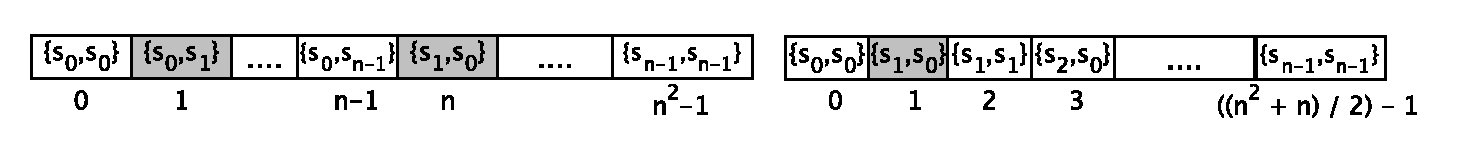
\includegraphics[width=\textwidth]{figs/memory.pdf}
	\caption{Indexing and placement of the state pair arrays. A simple placement of the pairs (on the left) uses redundant places for state pairs $\{s_i, s_j\}$, $i \neq j$, e.g., $\{s_1, s_2\}$ and $\{s_2, s_1\}$ in the figure. On the right, the indexing mechanism we used is shown.}
	\label{fig:mem}
\end{figure}

At the hardware level, a CUDA capable GPU processor is a collection of
\textit{multiprocessors} (SMX), each having a number of
\textit{processors}.  Each multiprocessor has its own shared memory
which is common to all its processors.  It also has a set of
registers, texture memory (a read only memory for the GPU), and
constant (a read only memory for the GPU that has the lowest access
latency) memory caches.  In any given cycle, each processor in the
multiprocessor executes the same instruction on different data.
Communication between multiprocessors can be achieved through the
\textit{global device memory}, which is available to all the
processors in all multiprocessors~\cite{nvidia}.

In the software level, the CUDA model is a collection of threads
running in parallel.  The programmer decides on the number of threads
to be launched.  A collection of threads, called a \textit{warp},
running simultaneously (on a multiprocessor).  If the number of
threads is more than the warp size then these threads are time-shared
internally on the multiprocessor.  At a given time, a \textit{block}
of threads runs on a multiprocessor.  Therefore a threads in block may
have bundled into several number of warps.  Each thread executes a
piece of code called a \textit{kernel}.  The kernel is the core code
to be executed on a multiprocessor.  During its execution, a thread
$t_i$ is given a unique ID and during execution thread $t_i$ can
access data residing in the GPU by using its ID.  Since the GPU memory
is available to all the threads, a thread can access any memory
location.  During GPU computation the CPU can continue to operate.
Therefore the CUDA programming model is a hybrid computing model in
which a GPU is referred as a co-processor (\textit{device}) for the
CPU (\textit{host}).

Due to architecture of GPU, algorithms that require less synchronization are more efficient. Since the number of threads too high, creating frontier and remaining sets is an inefficient operation. Therefore we implemented S2R and S2F algorithms. For CUDA version, each thread checks only one pair. To match pairs and threads, memory indexing formula is used.  requires synchronization to find global minimum.

For CUDA implementation of Algorithm \ref{algo:find-min-parallel} we used constant amount of threads. Each threads uses memory indexing formula to check pairs and finds the local minimum, like in S2R and S2F. When threads finds the local minimum it uses {\tt atomicMin} operation instead of sequential synchronization. 



%%%%%% SPEEDING UP THE FASTEST %%%%%% 
\clearpage
\section{Speeding up the Fastest}
\label{sec:speedup}

As mentioned in Section \ref{sec:greedy}, \greedyAlgo\ algorithm has two main phases: PMF construction and reset word generation via merging sequences. The observations from Section \ref{sec:greedy-analysis} shows that the first phase dominates the execution time of the algorithm. However, the second phase does not use all merging sequences to construct the reset word. Therefore the second phase can use a partial PMF. Hence, we propose three algorithmic enhancements for \greedyAlgo\ algorithm. As the first improvement a partial PMF construction runs in a lazy manner, which is introduced in Section \ref{sec:lazy}. Section \ref{sec:lookahead} explains the second proposal about searching the merging sequences from current pair in the latest stages. Last suggestion optimize the comparing of constructed BFS tree and set of current pair.  

\subsection{Lazy PMF Construction}
\label{sec:lazy}

\greedyAlgo\ algorithm uses PMF to pick the shortest merging sequence among the set of current pairs ($C^{\langle2\rangle}$). However, Table \ref{table:levels} shows that the algorithm does not need to construct all PMF. It is redundant to compute the merging sequences whose length is longer than $h_{max}$. As the first improvement, we generated PMF in a lazy way and combined the two phases. Algorithm \ref{algo:greedy-lazy} searches the shortest merging sequence in PMF which is also the shortest merging sequence of a pair in $C^{\langle2\rangle}$. The \greedyAlgo\ algorithm uses partial PMF which initially has only the merging sequences of the singletons. At each iteration, PMF is computed when it is needed. The algorithm checks all pairs in $C^{\langle2\rangle}$ to find the shortest merging sequence. If it cannot find the merging sequence then PMF construction phase is executed. It computes until a pair in $C^{\langle2\rangle}$ is found. After that it applies the merging sequence to all active pairs and process the next iteration. Note that BFS algorithm is used for PMF construction. Hence the length of not computed merging sequences cannot be shorter than any other computed merging sequence in PMF.
 
\begin{algorithm}[ht]	
	\caption{\greedyAlgo\ algorithm with lazy PMF construction}
	\label{algo:greedy-lazy}
	
	\SetKwInOut{Input}{input}\SetKwInOut{Output}{output}
	\Input{An automaton ${\cal A}=(S,\Sigma,\delta)$}
	\Output{A synchronizing word $\Gamma$ for ${\cal A}$}
	\lForEach{singleton $\{ s,s \} \in S^{\langle 2 \rangle}$}{$\tau(\{s,s\}) = \varepsilon$}
	\lForEach{pair $\{ s_i,s_j \} \in S^{\langle 2 \rangle}$}{$\tau(\{ s_i,s_j \})${\em undefined}}
	$Q \longleftarrow \{ \{ s,s \}| s \in S \}$; \tcp{Q is a queue which will store unprocessed pair from frontier set and found pair from next frontier set.}
	$C = S$; \tcp{$C$ will keep track of the current set of states}
	$\Gamma = \varepsilon$; \tcp{$\Gamma$ is the synchronizing sequence to be constructed}
	\While{$|C| > 1$}	
	{
		\While{$\forall \{ s_i,s_j \} \in C^{\langle 2 \rangle}: \tau(\{ s_i,s_j \})$ is undefined}
		{
			$\{ s_i, s_j \} = $ dequeue the next item from $Q$\;
			\ForEach{$x \in \Sigma$}
			{
				\ForEach{$\{ s_k, s_\ell \} \in \delta^{-1}(\{ s_i, s_j \},x)$}
				{
					\If{$\tau(\{ s_k, s_\ell \})$ is undefined}
					{
						$\tau(\{ s_k, s_\ell \}) = x \; \tau(\{ s_i, s_j\})$\;
						enqueue $\{ s_k,s_\ell \}$ onto $Q$\;
					}
				}
			} 		
		}
		find a pair $\{ s_i, s_j \} \in C^{\langle 2 \rangle}$ 
		with minimum $|\tau(\{ s_i,s_j \})|$ among all pairs 
		in $C^{\langle 2 \rangle}$\;
		$\Gamma = \Gamma \; \tau(\{ s_i, s_j \})$\;
		$C = \delta(C,\tau(\{ s_i,s_j\}))$;
	}
\end{algorithm}

Algorithm \ref{algo:greedy-lazy} has the same upper bound compared to Algorithm \ref{algo:greedy}. For line 7-13, the time complexity depends on the number of edges, $O(pn^2)$. The number of iterations does not effect the upper bound of Line 7-13. Also there is no lower bound for PMF construction part. Picking the shortest merging sequence (Line 14-16) is the same as in Algorithm \ref{algo:greedy}. Therefore the complexity is $O(n^4+ pn^2)$ and $\Omega(n)$. Thus the upper bound does not change but the lower bound decreases.

\subsection{Looking Ahead From Current Pair}
\label{sec:lookahead}

As noted in Section \ref{sec:lazy}, \greedyAlgo\ algorithm does not need a fully constructed PMF to find a short synchronizing sequence. Table \ref{table:levels} also shows that the average length of selected merging sequences are less than two. Hence, for the most iteration, the algorithm picks the merging sequence with the length of one. The algorithm occasionally picks a merging sequence with longer length, like $h_{max}$. So, Algorithm \ref{algo:greedy-lazy} has to construct PMF upto $h_{max}$ for only occasional cases. In this section, \textit{lookahead} approach is introduced to avoid constructing deep levels of PMF. 

\begin{algorithm}[ht]
	\caption{Looking ahead from $C^{\langle 2 \rangle}$}
	\label{algo:lookahead}
	
	\SetKwInOut{Input}{input}\SetKwInOut{Output}{output}
	\SetVlineSkip{0.1em}
	\setcounter{AlgoLine}{5}
	\nlset{$\mathbf{1..6}$} $\ldots$ \tcp{same as Algorithm~\ref{algo:greedy-lazy}} 
	\While{$|C| > 1$}	{
		\If{$\forall \{ s_i,s_j \} \in C^{\langle 2 \rangle}: \tau(\{ s_i,s_j \})$ is undefined} {
			\If{$|C| < $\sc{MaxStates}} {
				let $Q_L = C^{\langle 2 \rangle}$ and $Q_{L_2} = \emptyset$ be two queues\;	
				$q_{min} = \min_{\{ s_i, s_j \} \in Q} |\tau(\{ s_i, s_j \})|$; \\
				$cnt = 0$\;
			 	$\{ s_{k'},s_{\ell'}\}=$  {\em undefined}\;
			 	$\{ s_{k'_{root}},s_{\ell'_{root}}\}=$  {\em undefined}\;
				\lForEach{$\{ s_i, s_j \} \in S^{\langle 2 \rangle}$}{ $\sigma(\{ s_i, s_j \})  =$ {\em undefined}}
				\lForEach{$\{ s_i, s_j \} \in C^{\langle 2 \rangle}$}{$\sigma(\{ s_i, s_j \}) = \varepsilon$ and ${\{ s_{i_{root}},s_{j_{root}}\}}=\{s_i, s_j\}$}
				\While{$Q_L$ is not empty}{
					$\{ s_i, s_j \} = $ pop an item from $Q_L$\;\
				 	\For{$x \in \Sigma$} { 
						$\{ s_k, s_\ell \}$ = $\{ \delta(s_i,x), \delta(s_j,x)  \}$\;
						\If{$\sigma(\{ s_k, s_\ell \})$ is undefined}{
							push $\{ k, \ell \}$ to $Q_{L_2}$\;
							$\sigma(\{ s_k, s_\ell \}) = x \sigma(\{ s_i, s_j \})$\;
							${\{ s_{k_{root}}, s_{\ell_{root}} \}} = \{ s_{i_{root}}, s_{j_{root}} \}$\;
							$cnt++$;
						}
						\If{$\tau(\{ s_k, s_\ell \})$ is defined and $|\tau(\{ s_k, s_\ell \})| < |\tau(\{ s_{k'}, s_{\ell'} \})|$}{
							$\{ s_{k'}, s_{\ell'} \} = \{ s_k, s_\ell \}$	
						}
					}
					\If{$Q_L$ is empty and $cnt < ${\sc MaxPairs} and $\{ s_{k'},s_{\ell'}\}$ is undefined}{
						$Q_L = Q_{L_2}$ and $Q_{L_2} = \emptyset$;
					}
				}
				\If{${\{ s_{k'},s_{\ell'}\}}$ is defined}{
					use $\{ s_{k'_{root}},s_{\ell'_{root}}\}$ as $\{ s_i,s_j\}$ and $\sigma(\{ s_{k'}, s_{\ell'} \}) \tau(\{s_{k'},s_{\ell'} \})$ as $\tau(\{s_i,s_j \})$ for line 32-41
				}
			}
        	\While{$\forall \langle s_i,s_j \rangle \in C^{\langle 2 \rangle}: \tau(\{s_i,s_j \})$ is undefined} { 
        		\setcounter{AlgoLine}{37}
				\nlset{$\mathbf{33..38}$} $\ldots$ \tcp{same as lines 8-13 of Algo.~\ref{algo:greedy-lazy}}
			}
		}
		\setcounter{AlgoLine}{40}
		\nlset{$\mathbf{39..41}$} $\ldots$ \tcp{same as lines 14-16 of Algo.~\ref{algo:greedy-lazy}}
	}
\end{algorithm}

The lookahead approach tries to find a shortest path from $C^{\langle 2 \rangle}$ to $Q$ via $\delta$~(instead of $\delta^{-1}$). Let $\sigma_{\{  s_i, s_j \}}$ be the shortest path to $\{  s_i, s_j \}$ found by the lookahead PMF
started from $C^{\langle 2 \rangle}$. Algorithm~\ref{algo:lookahead} and Figure~\ref{fig:lookahead} summarize the basic lookahead process. 

When $\forall \langle s_i,s_j \rangle \in C^{\langle 2 \rangle}: \tau(\{s_i,s_j \})$ is undefined, applying lookahead approach fully and every time will be costly. To reduce the overhead, two constraints are defined; looking ahead is avoided when there are more than {\sc MaxStates}~(line 9)  states in $C$ and the process is allowed to traverse at most {\sc MaxPairs}~(line 16). We did not fine tune these parameters and use {\sc MaxStates} $= \log n$ and {\sc MaxPairs} $= n$. 

We never reuse the lookahead paths $\sigma(\{ i, j \})$ from the previous iteration (see lines 15-16 in Algorithm~\ref{algo:lookahead}); although, some bookkeeping can be applied. We forget all the lookahead information once the process ends, because we want to continue exploring the forest level-by-level in a BFS fashion to keep the paths being shortest during the course of the overall heuristic. 



\begin{figure}[ht]
	\centering
	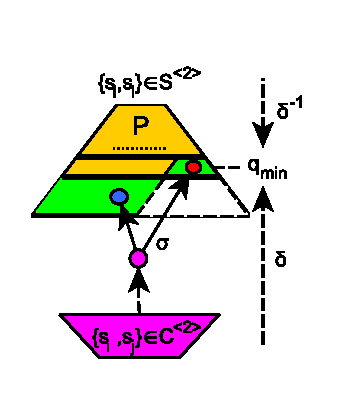
\includegraphics{figs/la.pdf}
	\caption{The figure summarizes the lookahead process: The BFS forest~(the top part of the figure) is being constructed via $\delta^{-1}$ in a lazy way. However, $P = \{ \{s_i, s_j \} | \tau(\{s_i, s_j \})~ \mbox{\em is defined} \}$ and $C^{\langle 2 \rangle}$ are disconnected. The process tries to find a shortest path from $C^{\langle 2 \rangle}$ to the queue $Q$~(the green colored BFS frontier). As an example, the $\sigma$ path passing through the blue $Q$ pair on the left is not the shortest one since there is a red $Q$ pair on the right which is reachable from the same purple lookahead pair. When the blue node is found, the current lookahead level (consisting of the nodes in $Q_L$) shall be completed to guarantee that the red node does (or does not) exist.}
	\label{fig:lookahead}
\end{figure}



\subsection{A Smart Way to Find the Intersection of Active Pair and Constructed PMF}
\label{sec:smart}

In Algorithm \ref{algo:greedy-lazy} and \ref{algo:lookahead}, the heuristic frequently checks if $\forall \{ s_i,s_j \} \in C^{\langle 2 \rangle}: \tau(\{ s_i,s_j \})$ is undefined or not. Our baseline implementation always traverses the pairs in $C^{\langle 2 \rangle}$ and checks if they are in $P = \{ \{s_i, s_j \} | \tau(\{s_i, s_j \})~ \mbox{\em is defined} \}$. Although this is efficient when $|C^{\langle 2 \rangle}|$ is small, $|C^{\langle 2 \rangle}|$ is not small enough at the early stages of the algorithm. Hence we reverse the search when $|C^{\langle 2 \rangle}| > |P|$ and traverse the pairs in $P$ and check if they are in $C^{\langle 2 \rangle}$.





%%%%%%%%%%%%%% RESULTS %%%%%%%%%%%%%%  
\clearpage
\section{Experimental Results}
\label{sec:results}

All the experiments in the thesis are performed on a single machine running on 64 bit CentOS 6.5 equipped with 64GB RAM and a dual-socket Intel Xeon E7-4870 v2 clocked at 2.30 GHz where each socket  has 15 cores~(30 in total). The machine also has a Nvidia K40 GPU with 12GB of global memory and 15 SMs each having 192 cores. For the multicore implementations, we used OpenMP and all the codes are compiled with {\tt gcc 4.9.2} with the {\tt -O3} optimization flag enabled and GPU parallelization is achieved with CUDA. All the codes are compiled with {\tt gcc 4.9.2} with the {\tt -O3} optimization flag enabled.

\sloppy
To measure the efficiency of the proposed algorithms, we used randomly generated automatons\footnote{For each state $s$ and input $x$, $\delta(s,x)$ is randomly assigned to a state $s' \in S$.} with $n  \in \{2000, 4000, 8000\}$ states and ${p \in \{2, 8, 32, 128\}}$ inputs. For each $(n, p)$ pair, we randomly generated $100$ different automatons and executed each algorithm on these automatons. The values in the figures and the tables are the averages of these $100$ executions for each configuration, i.e., algorithm, $n$ and $p$. As slowly synchronizing automata, we also used \v{C}ern\'y automata with $n  \in \{2000, 4000, 8000\}$ states. Since there is only one automaton for each $n$, for more reliable results we execute the algorithms 5 times for each $n$ value.

\subsection{Multicore Parallelization of PMF Construction}

For comparison, we implemented Algorithm in Section \ref{algo:greedy}, which is called sequential in this section. As CPU parallelization, we used the algorithms in Section \ref{sec:BFS-F2R-parallel}, \ref{sec:BFS-R2F-parallel} and \ref{sec:BFS-Hybrid-parallel} and tested with 1,2,4,8 and 16 threads. To observe the effect of the indexing formula, we implemented GPU parallelization with basic and memory optimized indexing functions. We called these two implementations as CUDA and CUDA M.O. respectively.

Figure~\ref{fig:f2r-speedup} shows the speedups of our parallel F2R implementation over the sequential baseline~(that has no parallelism). Since F2R uses the same frontier extension mechanism with the sequential baseline, whereas R2F, S2R and S2F employ completely different ones, here we only present the speedup values of F2R. As the figure shows, when $p$ is large, the parallel F2R presents good speedups, e.g., for $p = 128$, the average speedup is $13.4$ with $16$ threads. Furthermore, when compared to the single-thread F2R, the average speedup is $14.9$ with $16$ threads. A performance difference between sequential baseline and single-threaded F2R exists because of the parallelization overhead during the local queue management. Overall, we observed $10\%$ parallelization penalty for F2R on the average over the sequential baseline for all $(n, p)$ pairs. \comment{sertac}{penalty hesaplarken sadece 1 threadle mi karsilastirmak lazim?}

\begin{figure}[ht]
	\centering
	\subfigure[$n = 2000$]{
		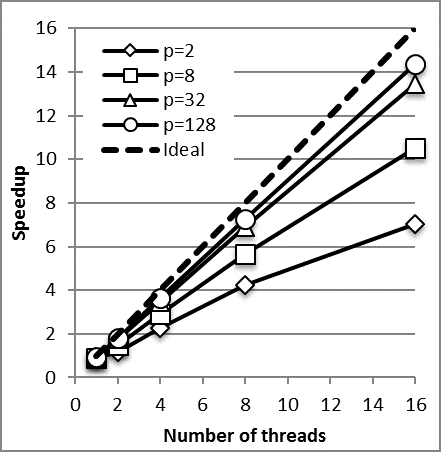
\includegraphics[height=0.33\textheight]{figs/spF2R_2000.png}
	}
	\subfigure[$n = 4000$]{
		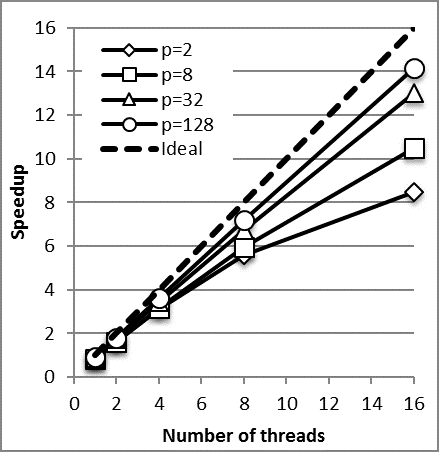
\includegraphics[height=0.33\textheight]{figs/spF2R_4000.png}
	}
	\subfigure[$n = 8000$]{
		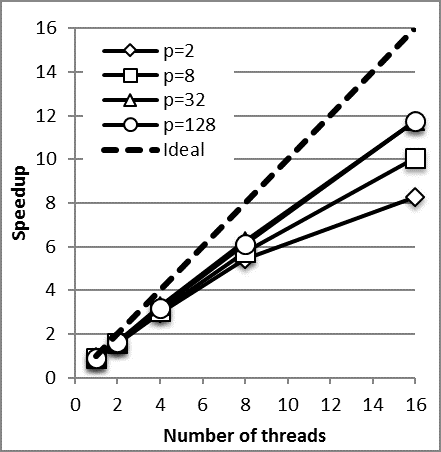
\includegraphics[height=0.33\textheight]{figs/spF2R_8000.png}
	}
	\caption{The speedup of our parallel F2R PMF construction over the sequential PMF construction baseline.}
	\label{fig:f2r-speedup}
\end{figure}

For $p$ values smaller than $128$, i.e., $2$, $8$, and $32$, the average speedups are $7.9$, $10.4$,  and $12.7$, respectively, with $16$ threads. The impact of the parallelization overhead is more for such cases since the amount of the local-queue overhead is proportional to the number of states but not to the number of edges. Consequently, when $p$ decreases the amount of total work decreases and hence, the impact of the overhead increases. Furthermore, since the number of iterations for PMF construction increases with decreasing $p$, the local queues are merged more for smaller $p$ values. Therefore, one can expect more overhead, and hence, less efficiency for smaller $p$ values as the experiments confirm.

\setlength{\tabcolsep}{3pt}
\begin{table}[ht]
	\centering
	\begin{spacing}{1.2}
		\scalebox{0.75}{
			\begin{tabular}{rr|rrrr|rrrr|rrrr}
				\multicolumn{1}{c}{} & \multicolumn{1}{c|}{} & \multicolumn{4}{c|}{n=2000} & \multicolumn{4}{c|}{n=4000} & \multicolumn{4}{c}{n=8000} \\
		
				\multicolumn{1}{c}{} & \multicolumn{1}{c|}{p} & \multicolumn{1}{c}{2} & 		\multicolumn{1}{c}{8} & \multicolumn{1}{c}{32} & \multicolumn{1}{c|}{128} & \multicolumn{1}{c}{2} & \multicolumn{1}{c}{8} & \multicolumn{1}{c}{32} & \multicolumn{1}{c|}{128} & \multicolumn{1}{c}{2} & \multicolumn{1}{c}{8} & \multicolumn{1}{c}{32} & \multicolumn{1}{c}{128} \\ \hline
		 
		 		& sequential & 0.17 & 0.50 & 2.11 & 9.13 & 1.18 & 2.71 & 9.92 & 40.36 & 5.90 & 14.29 & 51.78 & 193.55 \\ \hline
		
			\multirow{3}{*}{1} & F2R & 0.19 & 0.56 & 2.31 & 9.89 & 1.35 & 3.21 & 11.24 & 44.57 & 6.43 & 16.01 & 56.71 & 219.46 \\
		 
		 		& R2F & 0.59 & 0.46 & \textbf{0.85} & 1.91 & 3.17 & 2.61 & 4.72 & 11.39 & 19.41 & 18.17 & 34.35 & 86.60 \\

		 		& Hybrid & \textbf{0.14} & \textbf{0.18} & 0.96 & \textbf{0.65} & \textbf{1.06} & \textbf{0.89} & \textbf{2.99} & \textbf{1.92} & \textbf{5.16} & \textbf{8.42} & \textbf{8.93} & \textbf{5.80} \\ \hline

				\multirow{3}{*}{2} & F2R & 0.15 & 0.34 & 1.21 & 5.00 & 0.73 & 1.68 & 5.74 & 22.41 & 3.82 & 9.14 & 31.40 & 120.23 \\

				& R2F & 0.37 & 0.27 & \textbf{0.46} & 0.98 & 2.00 & 1.55 & 2.62 & 6.04 & 13.73 & 11.96 & 21.54 & 52.67 \\

			& Hybrid & \textbf{0.12} & \textbf{0.14} & 0.53 & \textbf{0.37} & \textbf{0.58} & \textbf{0.50} & \textbf{1.57} & \textbf{1.01} & \textbf{3.09} & \textbf{4.86} & \textbf{5.10} & \textbf{3.34} \\ \hline

				\multirow{3}{*}{4} & F2R & 0.08 & 0.17 & 0.61 & 2.50 & 0.38 & 0.86 & 2.88 & 11.11 & 1.99 & 4.67 & 15.79 & 60.42 \\

				& R2F & 0.20 & 0.15 & \textbf{0.24} & 0.50 & 1.09 & 0.82 & 1.36 & 3.05 & 7.43 & 6.43 & 11.34 & 27.21 \\

				& Hybrid & \textbf{0.06} & \textbf{0.07} & 0.27 & \textbf{0.19} & \textbf{0.31} & \textbf{0.26} & \textbf{0.80} & \textbf{0.52} & \textbf{1.62} & \textbf{2.49} & \textbf{2.61} & \textbf{1.73} \\ \hline

				\multirow{3}{*}{8} & F2R & 0.04 & 0.09 & 0.31 & 1.26 & 0.21 & 0.46 & 1.47 & 5.60 & 1.09 & 2.49 & 8.31 & 31.55 \\

				& R2F & 0.11 & 0.08 & 0.12 & 0.25 & 0.64 & 0.45 & 0.71 & 1.55 & 4.36 & 3.68 & 6.36 & 14.91 \\

				& Hybrid & \textbf{0.03} & \textbf{0.04} & \textbf{0.14} & \textbf{0.10} & \textbf{0.17} & \textbf{0.15} & \textbf{0.42} & \textbf{0.28} & \textbf{0.89} & \textbf{1.34} & \textbf{1.39} & \textbf{0.93} \\ \hline

				\multirow{3}{*}{16} & F2R & \textbf{0.02} & 0.05 & 0.16 & 0.64 & 0.14 & 0.26 & 0.76 & 2.85 & 0.71 & 1.42 & 4.41 & 16.50 \\

				& R2F & 0.06 & 0.04 & 0.06 & 0.13 & 0.41 & 0.26 & 0.38 & 0.81 & 2.78 & 2.38 & 4.06 & 9.10 \\

				& Hybrid & \textbf{0.02} & \textbf{0.02} & \textbf{0.07} & \textbf{0.05} & \textbf{0.12} & \textbf{0.09} & \textbf{0.23} & \textbf{0.16} & \textbf{0.59} & \textbf{0.80} & \textbf{0.80} & \textbf{0.57} \\ \hline

				\multirow{3}{*}{CUDA} & S2R & \textbf{0.02} & \textbf{0.02} & 0.05 & 0.17 & \textbf{0.07} & 0.09 & 0.20 & 0.77 & \textbf{0.31} & 0.39 & 0.92 & 3.36 \\

				& S2F & 0.03 & 0.04 & 0.11 & 0.46 & 0.14 & 0.19 & 0.61 & 2.54 & 0.65 & 0.91 & 4.04 & 13.29 \\

				& Hybrid & \textbf{0.02} & \textbf{0.02} & \textbf{0.03} & \textbf{0.05} & 0.09 & \textbf{0.07} & \textbf{0.12} & \textbf{0.14} & 0.41 & \textbf{0.39} & \textbf{0.46} & \textbf{0.48} \\ \hline

				\multirow{3}{*}{CUDA M.O.} & S2R & \textbf{0.01} & 0.02 & 0.04 & 0.16 & \textbf{0.05} & 0.07 & 0.19 & 0.76 & \textbf{0.21} & 0.31 & 0.85 & 3.33 \\
		
				& S2F & 0.02 & 0.02 & 0.06 & 0.19 & 0.08 & 0.10 & 0.29 & 1.16 & 0.34 & 0.49 & 1.74 & 6.36 \\
		
				& Hybrid & \textbf{0.01} & \textbf{0.01} & \textbf{0.03} & \textbf{0.04} & 0.06 & \textbf{0.05} & \textbf{0.10} & \textbf{0.13} & 0.24 & \textbf{0.28} & \textbf{0.36} & \textbf{0.39}
			\end{tabular}
		}
	\end{spacing}
	\caption{Comparison of the parallel execution times of the PMF construction algorithms.}
	\label{table:PMF_time}
\end{table}
\setlength{\tabcolsep}{6pt}


Table~\ref{table:PMF_time} compares the execution times of F2R, R2F, S2R, S2F and Hybrid algorithm for $n \in {2000, 4000, 8000}$, $p \in \{2, 8, 32, 128\}$ and $\{1, 2, 4, 8, 16\}$ threads. An interesting observation is that F2R is consistently faster than R2F for $p = 2$, however, it is slower otherwise. This can be explained by the difference in the number of required iterations to construct PMF: when $p$ is large, the frontier expands very quickly and the PMF is constructed in less iterations, e.g., for $n = 2000$, the PMF is generated in $16$ iterations for $p = 2$, whereas only $7$ iterations are required for $p = 8$. Since each edge will be processed once, the runtime of F2R always increases with $p$, i.e., with the number of edges. However, since the frontier expands much faster, the total number of remaining~(R-)pairs processed by the R2F throughout the process will probably decrease. Furthermore, since when the frontier is large, while traversing the edge list of an R-pair, it is more probable to early terminate the traversal and add the R-pair to the next frontier earlier. Surprisingly,  when $p$ increases, these may yield a decrease in the R2F runtime~(observe the change from $p = 2$ to $p = 8$ in Table~\ref{table:PMF_time}). However, once the performance benefits of early termination are fully exploited, an increase on the R2F runtime with increasing $p$ is more probable since the overall BFS work, i.e., the total number of edges, also increases with $p$~(observe the change from $p = 8$ to $p = 32$ in Table~\ref{table:PMF_time}).

Observing such performance differences for R2F and F2R on automatons with different characteristics, the potential benefit of a Hybrid algorithm in practice is more clear. As Table~\ref{table:PMF_time} shows, the hybrid approach, which is just a combination of F2R and R2F, is almost always faster than employing a pure F2R or a pure R2F BFS-level expansion. Furthermore, we do not need parallelism to observe these performance benefits: the Hybrid approach works better even when a single thread is used at runtime. \footnote{Although one can implement F2R, R2F, and Hybrid sequentially, we do not have their sequential variants. With their OpenMP-based implementations, we expect $20\%$ parallelization overhead for both R2F and Hybrid as in F2R since the parallelization techniques employed in the implementations  are similar.}. For example, when $n = 8000$ and $p = 128$, the Hybrid algorithm is $38$ and $15$ times faster than F2R and R2F, respectively. For the same automaton set, the speedups due to hybridization of the process become $29$ and $16$ with $16$ threads on average.

\begin{figure}[ht]
	\centering
	\subfigure[$p = 2$]{
		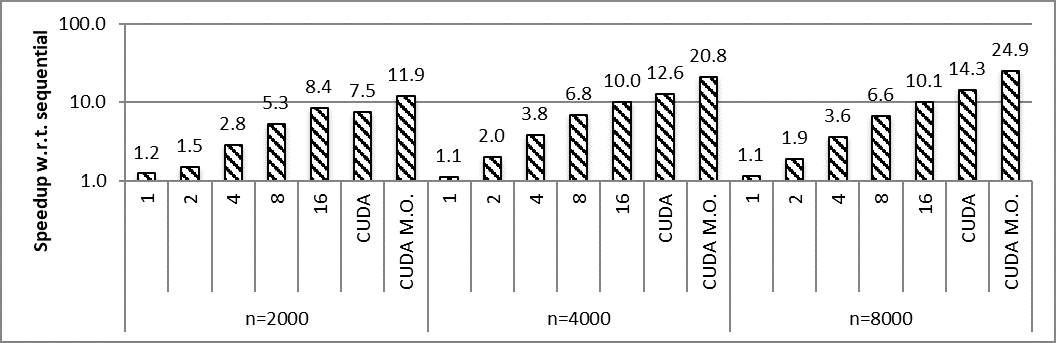
\includegraphics[height=0.17\textheight]{figs/hybrid_speedup_p2.png}
	}
	\subfigure[$p = 8$]{
		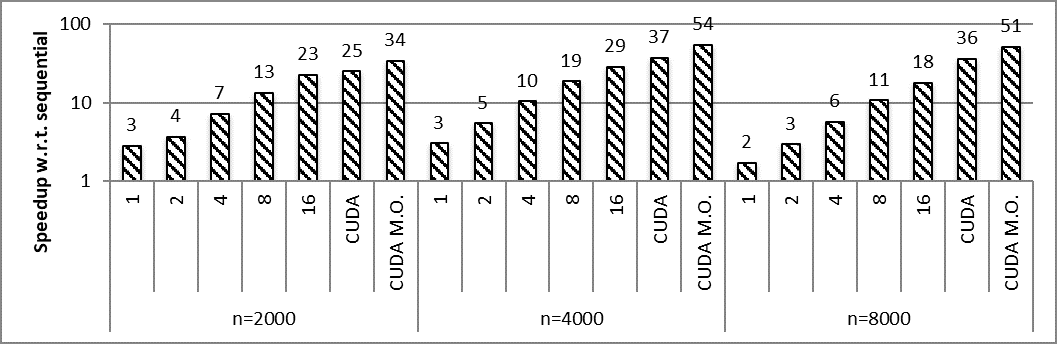
\includegraphics[height=0.17\textheight]{figs/hybrid_speedup_p8.png}
	}
	\subfigure[$p = 32$]{
		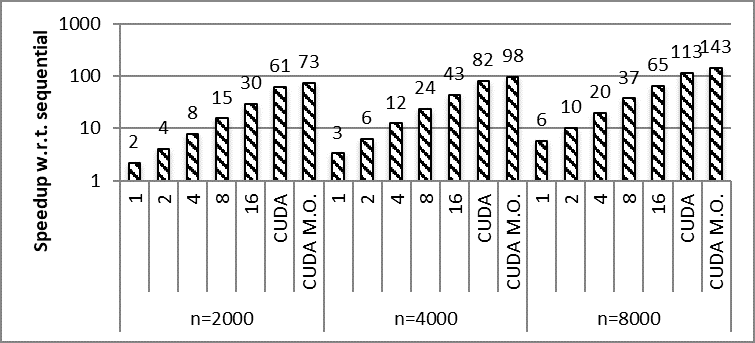
\includegraphics[height=0.17\textheight]{figs/hybrid_speedup_p32.png}
	}	
	\subfigure[$p = 128$]{
		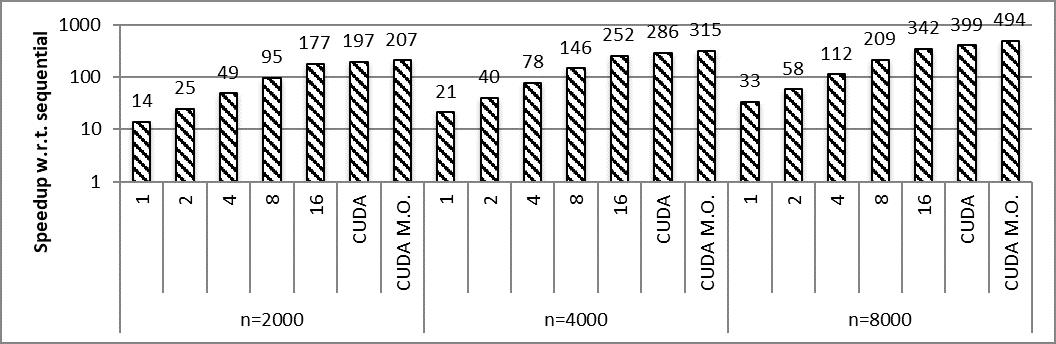
\includegraphics[height=0.17\textheight]{figs/hybrid_speedup_p128.png}
	}
	\caption{The speedups of the Hybrid PMF construction algorithms with $p = 2$~(top left), $8$~(top right), $32$~(bottom left), $128$~(bottom right) and $n \in \{2000, 4000, 8000\}$. The $x$-axis shows the number of threads used for the Hybrid execution.  The values are computed based on the average sequential PMF construction time over $100$ different automatons for each $(n, p)$ pair.}
	\label{fig:hybrid-speedup}
\end{figure}

When the Hybrid algorithm is used, the speedups on the PMF generation phase are given in Figure~\ref{fig:hybrid-speedup}. As the figure shows, thanks to parallelism and good scaling of Hybrid~(for large $p$ values), the speedups increase when the number of threads increases. The PMF generation process becomes $25$, $51$, $143$, and $494$ times faster when CUDA implementation with memory optimization used for $2$, $8$, $32$, and $128$ letter automatons, respectively.Even with single thread, i.e., no parallelization, the Hybrid heuristic is $33$ times faster than the sequential algorithm for $p=128$ and $n=8000$.

Since we generate the PMF to find a synchronizing sequence, a more practical evaluation metric would be the performance improvement over the sequential reset sequence construction process. As Table~\ref{table:phase-comparison} shows, for Eppstein's \greedyAlgo\ heuristic~(also for some other heuristics such as \textsc{Cycle}~\cite{Trahtman04}), the PMF generation phase dominates the overall runtime. For this reason, we simply conducted an experiment where the Hybrid approach is used to construct the PMF and no further parallelization is applied during the synchronizing sequence construction phase. Table~\ref{table:phase-comparison-after} shows the speedups for this experiment for single thread and $16$ thread Hybrid executions. As the results show, even when the sequence construction phase is not parallelized, more than $2$x and more than $14$x improvement is possible for $p = 32$ and $p = 128$, respectively.

\begin{table}[ht]
	\center
	\begin{tabular}{r|rrrr||rrrr}
		& \multicolumn{4}{c||}{Speedup} & \multicolumn{4}{c}{$\frac{t_{PMF}}{t_{ALL}}$}\\ 
		n\textbackslash p  & \multicolumn{1}{c}{2} & \multicolumn{1}{c}{8} & \multicolumn{1}{c}{32} & \multicolumn{1}{c||}{128} & \multicolumn{1}{c}{2} & \multicolumn{1}{c}{8} & \multicolumn{1}{c}{32} & \multicolumn{1}{c}{128} \\ \hline
		2000 & 11.90 & 34.20 & 72.99 & 206.84 & 0.52 & 0.53 & 0.69 & 0.77 \\
		4000 & 20.84 & 54.27 & 97.60 & 315.45 & 0.50 & 0.46 & 0.62 & 0.68 \\
		8000 & 24.92 & 51.00 & 143.01 & 493.97 & 0.36 & 0.39 & 0.45 & 0.47 
	\end{tabular}
	\caption{The speedups obtained on \greedyAlgo\ algorithm when the memory optimized CUDA implementation of Hybrid PMF construction algorithm is used.}
	\label{table:phase-comparison-after}
\end{table}

As noted before, F2R based PMF construction has $O(pn^2)$ time complexity. R2F based PMF construction, on the other hand, has $O(dpn^2)$ time complexity (where $d$ is the diameter of the pair automaton ${\cal A}$), since states of ${\cal A}$ in the remaining set $R$ will be processed at most $d$ times. In practice, however, R2F based construction (and Hybrid computation which also has $O(dpn^2)$ time complexity since it performs R2F steps) can beat F2R based construction.

We did not perform an extensive study on automata with larger state numbers, since it takes too long with the sequential baseline implementation. For example, sequential PMF generation takes around 2 hours and 30 minutes for an automaton with 40000 states and 128 letters, whereas our Hybrid implementation completes in 2 minutes and 30 seconds.

\subsection{Second Phase Parallelization}

As mentioned in Section \ref{sec:second-phase-parallelization}, execution time of second phase is worthy of note for only slowly synchronizing automata. Hence we used \v{C}ern\'y automata with $n \in \{ 2000, 4000, 8000 \}$ to compare our implementations. For CPU parallelization of second phase, we implemented the Algorithm \ref{algo:find-min-parallel} and tested with 1, 2, 4, 8 and 16 threads. For GPU parallelization we implemented the same algorithm with 256 thread per block and 256 block. We also implemented the approach that sorts the set of current pairs as mentioned in Section \ref{sec:implementation}.


\begin{table}[ht]
	\center
	\begin{tabular}{rr|rrr}
		& n & 2000 & 4000 & 8000\\\hline
		\multirow{2}{*}{sequential} & unsorted & 4.729 & 41.034 & 1035.093\\
		& sorted & 1.604 & 12.701 & 109.758\\\hline
		\multirow{2}{*}{1} & unsorted & 5.098 & 47.021 & 896.384\\
		& sorted & 2.553 & 20.274 & 168.116\\\hline
		\multirow{2}{*}{2} & unsorted & 3.869 & 37.352 & 874.253\\
		& sorted & 1.935 & 15.085 & 132.770\\\hline
		\multirow{2}{*}{4} & unsorted & 2.308 & 22.705 & 522.930\\
		& sorted & 1.178 & 8.946 & 75.673\\\hline
		\multirow{2}{*}{8} & unsorted & 1.259 & 13.131 & 289.750\\
		& sorted & 0.719 & 5.044 & 40.842\\\hline
		\multirow{2}{*}{16} & unsorted & 0.694 & 6.674 & 154.796\\
		& sorted & 0.723 & 3.350 & 22.403\\\hline
		\multirow{2}{*}{CUDA} & unsorted & 0.684 & 5.514 & 51.280\\
		& sorted & 0.391 & 1.556 & 9.613
	\end{tabular}
	\caption{Execution times of implementations of Algorithm \ref{algo:find-min} and \ref{algo:find-min-parallel}}
	\label{table:phase-2-time}
\end{table}

Table \ref{table:phase-2-time} shows that sorting the set of current pairs is a remarkable improvement. Even in sequential implementation we observed $3\times$ to $9.5\times$ speedups.

\subsection{Speeding up the Fastest}

We call the implementation of \greedyAlgo\ below as the naive baseline implementation. We also implemented the improvements over naive baseline as suggested in Section~\ref{sec:lazy}, Section~\ref{sec:lookahead}, and Section~\ref{sec:smart}. Below, we call these implementations as ``Lazy'', ``Lookahead'', and ``Smart'', respectively. Note that Lookahead is implemented on top of Lazy, and Smart is implemented on top of Lazy and Lookahead.


Figure~\ref{fig:speedups} presents the speedups of each improvement~(i.e. Lazy,  Lookahead, and Smart) over the naive baseline for \greedyAlgo . Lazy computation provides a stable improvement, which is more sensitive to alphabet size $p$. For a given alphabet size, we observe a somewhat constant speed up values. However, the average speedup values increase with the alphabet size. The lookahead also provides a stable improvement and it is more effective. For small alphabet sizes, the speedup provided by the lookahead is almost constant for different number of states. For larger alphabet sizes, on the other hand, the speedup provided by the lookahead increases with the number of states. The effect of the lookahead also increases with the alphabet size. The smart intersection check similarly improves the performance, but not to the same extent as lazy and lookahead.


\begin{figure}[ht]
	\centering
	\subfigure[$p = 2$]{
		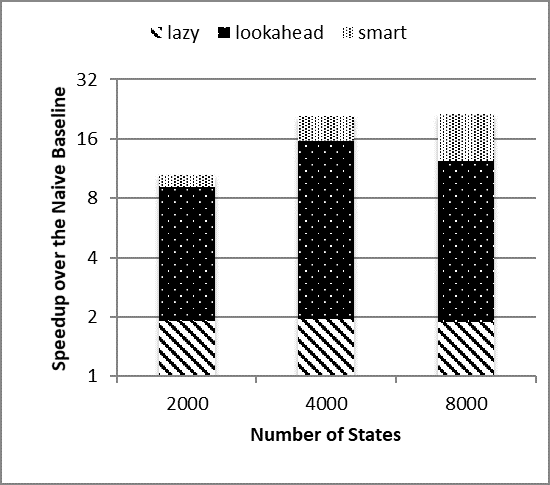
\includegraphics[width=0.47\textwidth]{figs/p2_greedy.png}
	}
	\subfigure[$p = 8$]{
		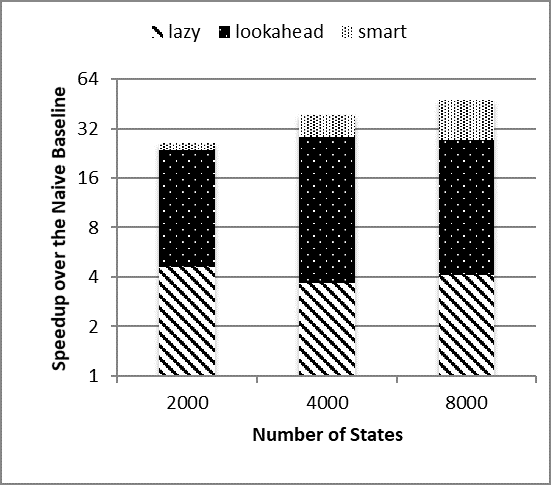
\includegraphics[width=0.47\textwidth]{figs/p8_greedy.png}
	}
	\subfigure[$p = 32$]{
		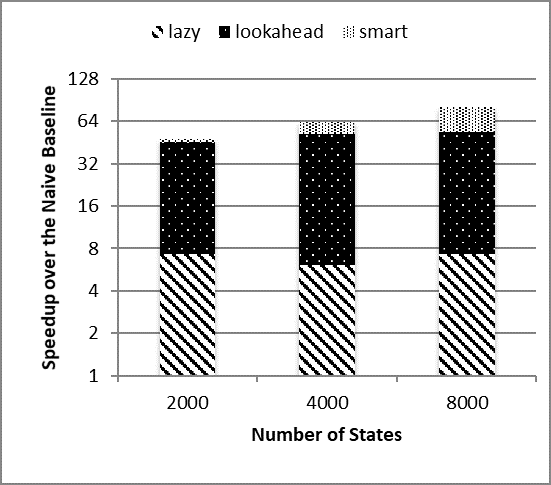
\includegraphics[width=0.47\textwidth]{figs/p32_greedy.png}
	}
	\subfigure[$p = 128$]{
		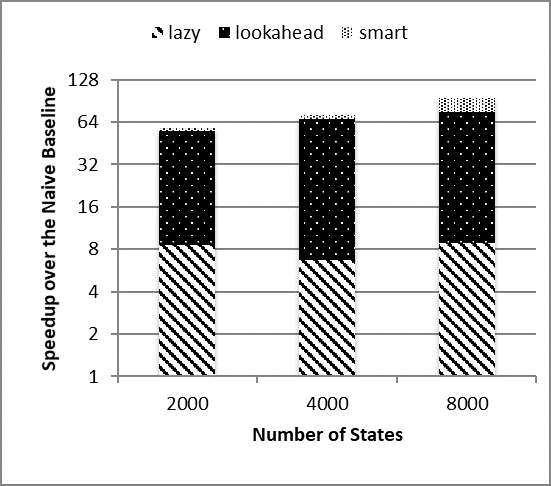
\includegraphics[width=0.47\textwidth]{figs/p128_greedy.png}
	}
	\caption{The speedup values normalized w.r.t. the naive baseline. For each additional improvement, the cumulative speedup is given with stacked columns.}
	\label{fig:speedups}
\end{figure}

Overall, when all the improvements are considered together, the average speedup values shows an increasing trend as the size of the automaton increases, and as we apply more aggressive improvements. We start with $2\times$ speedup for the automata with $n=2000$ and $p=2$ when only the lazy computation is enabled, and we reach to $95\times$ (almost two orders of magnitude) speedup for the automata with $n=8000$ and $p=128$ when all the improvements are enabled.

To validate effectiveness of our methods, we compare the time spent for BFS forest construction in each method. Note that, the time spent in PMF construction is proportional to the number of edges processed. The total number of edges to be processed for an automaton with $n$ states and $p$ letters is $pn(n-1)/2$. Table~\ref{table:edge-percent} reports the percentage of these edges processed by each method.

\begin{table}[ht]
	\center
	\begin{tabular}{rr||r||rrr}
$n$		&	$p$	& Algorithm~\ref{algo:BFS} 	& Lazy		& Lookahaed & Smart \\\hline\hline
2000	& 2		& 99.99\%					& 40.31\%	& 1.71\%	& 1.71\%\\
		& 8		& 84.83\%					& 12.18\%	& 0.56\%	& 0.57\%\\
		& 32	& 37.41\%					& 3.64\%	& 0.25\%	& 0.25\%\\
		& 128	& 11.19\%					& 1.00\%	& 0.11\%	& 0.09\%\\\hline
4000	& 2		& 99.99\%					& 36.92\%	& 1.42\%	& 1.52\%\\
		& 8		& 87.11\%					& 11.72\%	& 0.42\%	& 0.45\%\\
		& 32	& 40.12\%					& 2.93\%	& 0.16\%	& 0.17\%\\
		& 128	& 12.08\%					& 0.94\%	& 0.07\%	& 0.08\%\\\hline
8000	& 2		& 100.00\%					& 37.56\%	& 1.31\%	& 1.24\%\\
		& 8		& 89.16\%					& 12.09\%	& 0.38\%	& 0.33\%\\
		& 32	& 42.78\%					& 3.08\%	& 0.11\%	& 0.06\%\\
		& 128	& 13.02\%					& 0.83\%	& 0.06\%	& 0.05\%
	\end{tabular}
	\caption{The percentage of processed edges}
	\label{table:edge-percent}
\end{table}
First of all, note that even Algorithm~\ref{algo:BFS} does not process all edges. This is caused by the termination condition of the while--loop at line 5. In Algorithm~\ref{algo:BFS}, another possible termination is given at line 5 as a comment: ``$F$ is not empty''. When this alternative termination condition is used, Algorithm~\ref{algo:BFS} processes 100\% of the edges. 

Recall that the initial motivation for this work is based on the observation that PMF construction time being too high compared to the overall running time of \greedyAlgo . We aimed at reducing this high cost, by modifying \greedyAlgo\ so that they can run without full PMF construction. The figures in Table~\ref{table:edge-percent} show that we succeed. Only a very small part of the PMF is constructed in the modified version of \greedyAlgo Algorithm. As the size of the automata increases, the percentage of the PMF constructed decreases.

\clearpage
\section{Conclusion and Future Works}
\label{sec:conclusion}

\textsc{Greedy} is widely used as a performance baseline for the new heuristics in the literature. None of the newer heuristics could actually match the time performance of \textsc{Greedy} and \textsc{Cycle} so far. With the new improved approaches suggested in this thesis, \textsc{Greedy} and \textsc{Cycle} have now become more competitive than they already are.


We investigated the efficient implementation and use of modern multicore CPUs and GPUs to scale the performance of synchronizing sequence generation heuristics. We parallelized one of the well-known heuristics \textsc{Greedy}. We mainly focused on the PMF generation phase (which is employed by almost all the heuristics in the literature), since it is the most time consuming part of \textsc{Greedy}. Even with no parallelization, our algorithmic improvements yielded a 33x speedup on \textsc{Greedy} for automatons with 8000 states and 128 inputs. Furthermore, around 494x speedup has been obtained with GPU parallelization for the same automata class.

First phase of \greedyAlgo\ is common for the well known synchronizing heuristics, such as  \textsc{SynchroP}, \textsc{SynchroPL}, and \textsc{FastSynchro}. Although the first phase does not dominates, parallelization techniques can be applied to other heuristics. One can also parallelize second phase of the  slower heuristics to make them more competitive.  

Furthermore, we proposed techniques to speedup the synchronizing heuristics \textsc{Greedy}. This is accomplished by first removing the quadratic lower bound for the running time of these heuristics. Using additional optimizations, we obtained order(s) of magnitude speed up values for \textsc{Greedy}.
The techniques suggested in this thesis become more effective as the size of the automata increases. Due to the increased speeds of \textsc{Greedy}, these heuristics will now scale more.


Note that other synchronizing heuristics existing in the literature such as \textsc{SynchroP}, \textsc{SynchroPL}, and \textsc{FastSynchro} cannot directly benefit from the lazy computation and further techniques. 
These heuristics require shortest merging sequence information for many pairs of states, if not for all. Due to this property, a large part of, or the entire, BFS forest
will have to be constructed. Therefore, the underlying intuition for  \textsc{SynchroP}, \textsc{SynchroPL}, and \textsc{FastSynchro} will need to be changed in order for them to take advantage of the algorithmic improvements that the thesis proposed. Modifying the underlying intuition for \textsc{SynchroP}, \textsc{SynchroPL}, and \textsc{FastSynchro} so that they can also benefit from the techniques suggested in this thesis can be considered as a future work.


\clearpage
\bibliographystyle{plain}
\bibliography{thesis}

\end{document}


